\documentclass[oneside,a4paper,12pt]{article} % Gibt an: Papierformat, Schriftgröße

\usepackage{thesis}
\usepackage{amsmath}
\usepackage{algorithm}
\usepackage[noend]{algpseudocode}
\usepackage{subfig}

%UML
\usepackage[T1]{fontenc}
\usepackage{tikz-uml}

%Code
\usepackage{listings}
\usepackage{xcolor}

%calc
\usepackage{calc}

%array
\usepackage{array}

%svg
\usepackage{svg}




\definecolor{codegreen}{rgb}{0,0.6,0}
\definecolor{codegray}{rgb}{0.7,0.7,0.7}
\definecolor{codekit}{rgb}{0.281,0.441,0.402}
\definecolor{backcolour}{rgb}{0.93,0.953,0.949}
\definecolor{codeblue}{rgb}{0.246,0.352,0.602}

\lstdefinestyle{codeStyle}{
    backgroundcolor=\color{backcolour},   
    commentstyle=\color{codegreen},
    keywordstyle=\color{codeblue},
    numberstyle=\tiny\color{codegray},
    stringstyle=\color{codekit},
    keywordsprefix={@},
    basicstyle=\ttfamily\footnotesize,
    breakatwhitespace=false,         
    breaklines=true,                 
    captionpos=b,                    
    keepspaces=true,                 
    numbers=left,                    
    numbersep=5pt,                  
    showspaces=false,                
    showstringspaces=false,
    showtabs=false,
    tabsize=2
}

\lstset{style=codeStyle}






% Hier werden die Abkürzungen definiert. Sofern ein Abkürzungsverzeichnis verwendet wird bitte entkommentieren.
\newacronym{iot}{IoT}{Internet of Things}
\newacronym{aifb}{AIFB}{Institut für Angewandte Informatik und Formale Beschreibungsverfahren}
\newacronym{kit}{KIT}{Karslruher Institute für Technologie}
\newacronym{vm}{VM}{Virtual Machines}
\newacronym{criu}{CRIU}{Checkpoint and Restore in Userspace}
\newacronym{cpu}{CPU}{Central Processing Unit}
\newacronym{csv}{CSV}{Comma Separated Values}
\newacronym{mib}{MiB}{Mebibyte (1024$^{2}$ Byte)}
\newacronym{dlac}{DLAC}{Dual Level Asynchronous Checkpointing}
\newacronym{gui}{GUI}{Graphical User Interface}
\newacronym{vas}{VAS}{virtual address spaces}
\newacronym{dram}{DRAM}{Dynamic Random Access Memory}
\newacronym{io}{IO}{Input/Output}
\newacronym{rest}{REST}{Representational State Transfer}
\newacronym{url}{URL}{Uniform Resource Locator}
\newacronym{rq}{RQ}{Research Question}
\newacronym{e}{E}{Experiment}
\newacronym{os}{OS}{Operating System}
\newacronym{pe}{PE}{Pipeline Element}
\newacronym{blcr}{BLCR}{Berkeley Lab Checkpoint/Restart}
\newacronym{sdk}{SDK}{Software Development Kit}

\begin{document}
\setlanguageEnglish % Sprache einstellen.

% Hier kommt der ganze Vorspann. Bei Verwendung von Abkürzungs-, Abbildungs- oder Tabellenverzeichnisse bitte in dieser Datei entsprechend entkommentieren.
\pagenumbering{roman}
\begin{titlepage}
% font / Schriftart
%------------------	


\begin{figure}[htbp]
  %\centering
  \begin{minipage}[b]{7cm}
    \ifthenelse{\boolean{english}}{
\includegraphics[height=1.8cm]{images/kit_logo_en}}{
\includegraphics[height=1.8cm]{images/kit_logo_de}}
  \end{minipage}
  \begin{minipage}[b]{8.5cm}
	\begin{flushright}


    
\includegraphics[height=1.8cm]{images/aifb_logo}  
		\end{flushright}
  \end{minipage}
\end{figure}

\vspace*{2.5cm}
\begin{center}
		%TODO Titel angeben
		{\textbf{\Huge \ifthenelse{\boolean{english}}{Adapting Stream Processing Pipelines in Fog Infrastructures}{Titel der Arbeit}}}
		\vspace*{1cm}\\
		%TODO Art der Arbeit
		{\Large \ifthenelse{\boolean{english}}{Bachelor Thesis}{Bachelorarbeit}}\\[0.5cm]
		{\Large \ifthenelse{\boolean{english}}{by}{von}}\\[1cm]
		%\vspace*{1cm}
		%TODO Name des Studenten
		{\Huge Daniel Gomm}\\[0.5cm]
		%TODO Studiengang des Studenten
		{\Large \ifthenelse{\boolean{english}}{Degree Course: Industrial Engineering and Management B.Sc.}{Studiengang: Wirtschaftsingenieurwesen}}\\[0.25cm]
		%TODO MatNr angeben
		{\Large \ifthenelse{\boolean{english}}{Matriculation Number}{Matrikelnummer}: 2055065}\\
		\vspace*{1.5cm}
		{\Large\ifthenelse{\boolean{english}}{
			Institute of Applied Informatics and Formal Description Methods (AIFB)
			\\[0.5cm]
			KIT Department of Economics and Management}{
			Institut für Angewandte Informatik und Formale Beschreibungsverfahren (AIFB)
			\\[0.5cm]
			KIT-Fakultät für Wirtschaftswissenschaften}
		}
	\end{center}
	\vspace*{1.5cm}
\Large{
\begin{center}
\begin{tabular}[ht]{l c l}
	
  %TODO Referent/-in angebenn
  %Referent/-in sind die Professoren, die die Arbeit bewerten.
  \ifthenelse{\boolean{english}}{Advisor}{Prüfer}: & \hfill  & Prof. Dr. York Sure-Vetter \\
  %Referent/-in sind die Professoren, die die Arbeit bewerten.
  \ifthenelse{\boolean{english}}{Second Advisor}{Zweiter Prüfer}: & \hfill  & Prof. Dr. Andreas Oberweis \\
  %TODO Betreuer/-in angeben
  \ifthenelse{\boolean{english}}{Supervisor}{Betreuer}: & \hfill  & M.Sc. Patrick Wiener \\
  %TODO Abgabedatum angeben
  \ifthenelse{\boolean{english}}{Submitted}{Eingereicht am}: & \hfill  & October 19, 2020\\
 
\end{tabular}
\end{center}

}


%\include{titel}
  \vfill
	
	\small{ KIT -- \ifthenelse{\boolean{english}}{The Research University in the Helmholtz Association}{Die Forschungsuniversität in der Helmholtz-Gemeinschaft}
} \hfill
	\small{\textbf{\url{www.kit.edu}} }
\end{titlepage}
%Für den Fall eines Vorworts entkommentieren:
%\mbox{}\thispagestyle{empty}

\vspace*{1cm}

{\Large \textbf{\ifthenelse{\boolean{english}}{Prologue}{Vorwort}}} 

\bigskip

\ifthenelse{\boolean{english}}
{\selectlanguage{english}
In English theses, German prologue is probably to be used, so paste it here. \blindtext
}
{\selectlanguage{ngerman}
Hier könnte ein Vorwort stehen.
}
\thispagestyle{empty}\section*{\ifthenelse{\boolean{english}}{Abstract}{Zusammenfassung}}

As the number of \acrfull{iot} devices continues to grow, means of effectively deploying \gls{iot} applications become increasingly important. Fog computing can provide an appropriate platform for many of these applications. A commonly deployed application in such a setting is stream processing. This thesis thus addresses the issue of adapting stream processing pipelines while they are running. Stream processing pipelines perform computations through a sequence of Pipeline Elements (\acrshort{pe}s). These \acrshort{pe}s can be deployed across different fog nodes. Adapting a stream processing pipeline thus refers to the relocation (migration) of \acrshort{pe}s between fog nodes. In the therefore developed conceptual framework, the two sub-problems migration of a correctly running \acrshort{pe} and migration of an interrupted \acrshort{pe} are handled separately and are addressed with respective procedures. These procedures were implemented into Apache StreamPipes (incubating) as a proof of concept. The evaluation of this proof of concept shows that the proposed procedures perform the migration consistently and with a low \acrshort{pe} downtime.




%Workload mobility can address a multitude of challenges that typically arise in fog computing, especially in the context of IoT applications. Addressing this issue, this work proposes an approach that allows for consistent migration of stateful stream processing \gls{pe}s in the fog. The two sub-problems migration of a correctly running \gls{pe} and migration of an interrupted \gls{pe} are handled separately and are addressed with corresponding procedures. These procedures were implemented into Apache StreamPipes (incubating) as a proof of concept. The evaluation of this proof of concept shows that the proposed procedures perform the migration consistently and with a low \gls{pe} downtime.


%An dieser Stelle erfolgt eine knappe Zusammenfassung der vorliegenden Arbeit ([engl.] Abstract), die maximal ca. 200 Worte umfassen sollte. Der Sinn und Zweck dieser Zusammenfassung liegt darin, einem interessierten Leser die Entscheidung zu erleichtern, die vorliegende Arbeit überhaupt zu lesen bzw. vor dem Lesen der Arbeit erst einmal in Erfahrung zu bringen, worum es dabei geht. Also eine knappe, motivierende Hinführung zum Problem und wie Sie es gelöst haben.

%Wenn Sie eine Zusammenfassung schreiben, bedenken Sie, dass diese oft auch alleine publiziert wird, d.h. sie sollte unabhängig vom nachfolgenden explizit dargestellten Inhalt der Arbeit für den Leser verständlich sein. Daher ist es immer sinnvoll, diese Zusammenfassung erst ganz am Ende zu schreiben, wenn Sie die eigentliche Arbeit bereits abgeschlossen haben.
%\setcounter{page}{3}
\tableofcontents\newcounter{roemisch} %\setcounter{roemisch}{\value{page}}
% Für den Fall von Abkürzungs-, Abbildungs- oder Tabellenverzeichnissen entkommentieren
\ifthenelse{\boolean{english}}
{\cleardoublepage\printnoidxglossary[type=acronym,sort=letter,nonumberlist,title={List of Abbreviations}]}
{\cleardoublepage\printnoidxglossary[type=acronym,sort=letter,nonumberlist,title={Abkürzungsverzeichnis}]}
\cleardoublepage\listoffigures
\cleardoublepage\listoftables
\cleardoublepage\setcounter{page}{2} 
\cleardoublepage
\pagenumbering{arabic}

% Füge hier die Kapitel per Verweis ein. Der Befehl \include fügt die angegebene tex-Datei an der jeweiligen Stelle ein. Die eingefügte Datei wird als normaler Teil des Quelltextes mitverarbeitet und ist daher LaTeX-Code (ohne Vorspann und \begin{document}...\end{document}).
\section{Introduction}
\label{lIntroduction}
While the concept of the \acrfull{iot} has been around for about 20 years \cite{Hutchison.2010}, mainstream attention and adoption have just recently seen a steep increase. Between 2012 and 2017, the annual search interest in \gls{iot} has increased more than nine-fold, according to data from Google (see Appendix \ref{lSearchInterestInIoT}). In the same timeframe, industrial adoption has grown as well. According to an industry report commissioned by Microsoft \cite{Microsoft.2020}, 91\% of the companies contacted were in the process of adopting \gls{iot} technologies in 2019. In addition, 64\% of the companies reported plans to further expand their \gls{iot} ventures in the next two years.\par
In parallel with this rise in interest and industrial adoption, the number of connected devices is expected to more than quadruple between 2015 and 2025, reaching more than 75 billion at the end of 2025 \cite{B.Safaei.2017}. With this ever-growing number of connected devices, the significance of effectively deploying these devices in \gls{iot} applications is growing as well. For effective deployment, several requirements must be fulfilled. These requirements were outlined by Yigitoglu et al. \cite{Yigitoglu.2017}. They are based on latency, bandwidth, resource constraints, mobility, dynamic workloads, multi-tenancy, and privacy. To deploy \gls{iot} devices and applications in line with these requirements, neither a solely cloud-based approach nor a solely edge-based one is appropriate \cite{Yousefpour.2019}. Thus, a combined approach of edge and cloud computing is needed.\\
The fog computing paradigm addresses this combination, extending cloud computing to the network edge \cite{Bonomi.2012}. The capabilities and characteristics of edge computing (e.g., low latency, real-time computing, etc.) and cloud computing (e.g., an abundance of computing resources, etc.) are combined in fog computing, making it a well-suited approach for most \gls{iot} applications \cite{Yousefpour.2019}.\\
Many tasks in the \gls{iot} context run continuously and can be divided into several consecutive steps. One way to address such a continuously running task comprised of a sequence of steps is through stream processing. In stream-processing, an input data stream is processed in a sequence of actions, forming a so-called stream processing pipeline. Each of these actions is executed by an action-specific processor, referred to as \acrfull{pe}. Besides the \gls{iot} context, stream processing is used in a variety of applications, including electronic trading, fraud control, and infrastructure monitoring \cite{Stonebraker.2005}.\\
Using fog computing and stream processing in combination can thus address commonly encountered tasks in the \gls{iot} within an \gls{iot} compatible frame. However, the deployment of stream processing applications in the fog comes with some challenges. To visualize these challenges, two illustrative cases are introduced. These cases also serve to illustrate the underlying technology, the addressed problems, and the developed conceptual framework in the subsequent chapters. While the first case is abstract and serves as an easy-to-follow example constructed for this thesis, the second case represents a real-world use case and is a simplified adoption for stream processing in the fog of the work of Chowdhurry et al. \cite{Chowdhury.2019}:\par

\begin{enumerate}[label=Case \arabic* , wide=0.5em,  leftmargin=*]
    \item \label{cAggregation} The first case is a simple example of a stream processing pipeline, which aggregates values. As depicted in Figure \ref{fExemplaryCases}, the stream processing pipeline gets its input data stream from a text file that contains numeric \gls{csv}. The second \gls{pe} aggregates incoming values over a predefined window of past events and passes on the result. In the last step, this data stream of values is written to a \gls{csv} output text file. Using this stream processing pipeline, the result's consistency can be monitored, and the functionality can be tested.
    \item \label{cMedical} The second case is based on a medical wearable device that monitors a patient’s electrocardiogram. Early symptoms of heart attacks are detected using the acquired electrocardiogram data. Therefore, the sensory data needs to be classified using a neural network, which can trigger an alarm on the patient’s wearable device. In detail, this application consists of 5 steps, as shown in Figure \ref{fExemplaryCases}. First, sensors acquire the data. Next, the signal is amplified, then filtered before the classification occurs. Finally, an alarm on the wearable device is triggered when symptoms are detected.
\end{enumerate}

\begin{figure}[H]
\graphicspath{{./figures/code/}}
\includesvg[width=\textwidth]{figures/visualizations/ExemplaryCases_1500.svg}
\caption{Stream processing pipelines of the illustrative cases}
\label{fExemplaryCases}
\end{figure}


The application in \ref{cMedical} requires a notable amount of computing resources for the classification of the sensory information. However its overall computing time should be as small as possible to alarm the patient in time to take necessary actions. At the same time, the wearable device has only limited computational capabilities and cannot provide sufficient service quality in the classification step. To cater to these needs, the task is realized as a stream processing pipeline deployed in the fog. Fog computing is utilized by deploying the \gls{pe}s individually and distributing them across fog nodes (different computing devices in the fog). To achieve a low latency, the \gls{pe}s for the computationally intensive steps are deployed on resource rich nodes with low latency in close vicinity. The \gls{pe} that inputs the electrocardiogram data into the stream processing pipeline, and the \gls{pe} that triggers the alarm are deployed on the wearable device. Due to wearable devices' mobile nature, the computing nodes in close vicinity are continually changing, thus requiring a possibility to relocate the pipeline's components while the pipeline is running. This dynamic relocation is referred to as workload-mobility \cite{Yigitoglu.2017}. Workload-mobility can also be important in the case of a resource scarcity at a node, which bottlenecks the application's computing time, and therefore imposes a significant toll on the application's usefulness. Additionally, in a situation in which a fog node hosting a \gls{pe} becomes unreachable, for example, because its network connection is interrupted, the \gls{pe} has to be relocated as well to facilitate the continuation of the pipeline's execution.\\
To address these challenges it is necessary to adapt stream processing pipelines while they are running by relocating \gls{pe}s. This relocation is referred to as migration. Migration means that processing previously performed on a specific node is shifted to another node. The migration also facilitates the fulfillment of the requirements for effective \gls{iot} deployment, which were introduced above. In detail, the migration provides means to better address latency, resource constraints, node mobility, dynamic workloads, and privacy.\par
This thesis focuses on developing a conceptual framework for the migration of stream processing applications in the fog. More precisely, this thesis focuses on the following research questions:

\begin{enumerate}[label=Research Question \arabic* , wide=0.5em,  leftmargin=*]
    \item \label{rqMigration} How can stateless and stateful event-driven \gls{pe}s be migrated between nodes in the fog?
    \item \label{rqConsistency} How can the data stream's consistent processing be facilitated when an event-driven \gls{pe} is migrated between nodes in the fog?
\end{enumerate}

By addressing these research questions, this thesis fills gaps in existing research. To the best of the author's knowledge, there has not been any prior research into the migration of stateful stream processing \gls{pe}s that considered the fog computing paradigm's specific challenges and opportunities.\\
Therefore, this thesis develops a conceptual framework for the migration of \gls{pe}s that also takes the specific challenges and opportunities of fog computing into account. Moreover, this thesis proposes separate migration tactics for different situations.\par
%Hier könnte ich mich auch alternativ von dem Teil zu der Contribution in Yigitoglu.2017 inspirieren lassen und meine Contribution ausführlich auflisten und den Ausblick dafür stark beschneiden 

The Second chapter lays the groundwork by focusing on the enabling technologies for this thesis, giving a high-level overview of fog computing and stream processing, emphasizing state.\\
The third chapter introduces related works that assess the migration of applications in the fog. It also considers works regarding the subject of state in data processing. The presented works propose differing approaches for the migration of applications and for state management.\\
In chapter \ref{lMethodology}, these approaches are compared, and the requirements for the migration of stream processing \gls{pe}s in the fog are outlined. However, the chapter's main focus is on the development of a conceptual framework for the migration of \gls{pe}s. The developed conceptual framework handles the migration of running and interrupted \gls{pe}s distinctly. For running \gls{pe}s, \textit{\acrshort{pe} live migration} is proposed, interrupted \gls{pe}s are relocated using the \textit{\acrshort{pe} restoration}. The \textit{\acrshort{pe} restoration} relies on centrally available \gls{pe} state checkpoints. To acquire these checkpoints, dual-level asynchronous checkpointing is introduced.\\
As a proof of concept, the developed conceptual migration approach is then implemented into Apache StreamPipes (incubating) in chapter \ref{lImplementation}. This chapter provides an in-depth overview of the concept's implementation and outlines implementation details of modifications and extensions of StreamPipes, presupposed by the conceptual framework.\\
The sixth chapter evaluates this implementation to assess whether and to which extent the requirements
for the conceptual framework are met. The chapter is closed by pointing out the limitations of the thesis.\\
The seventh chapter titled Conclusion, is the summary. Besides presenting conclusions it also outlines potential directions for further research.
\section{Background}
\label{lBackground}
This chapter introduces fog computing and stream processing. A profound understanding of both of these topics is needed as background for the subsequent chapters. Thus, fog computing is thoroughly introduced, defined, and its intricacies are pointed out. Furthermore, stream processing is introduced together with the concept of state in the stream processing context. State is then examined in detail, and relevant aspects in the handling of state are pointed out.

\subsection{Fog Computing}
\label{lFogComputing}
There are various definitions of the fog computing paradigm. In this thesis, the definition of Bonomi et al. \cite{Bonomi.2012} is used. They state that "fog computing extends the cloud computing paradigm to the edge of the network" \cite{Bonomi.2012}. They further describe fog computing as a highly virtualized platform that connects end devices with traditional cloud services by providing compute, storage, and networking services in between.\\
This definition of fog computing includes all available connected devices, meaning that compared to cloud computing, which typically solely utilizes large data centers \cite{Yousefpour.2019}, fog computing takes advantage of small servers, routers, switches, gateways, set-top boxes, and other small computing devices \cite{Yousefpour.2019} as well as the cloud infrastructure, which remains a core component.\par
To give a more comprehensive overview the characteristics that portray fog computing are presented in the following listing: 

\begin{itemize}
    \item Since a lot of the devices used in fog computing occupy a relatively small space, this hardware can be located close to the network edge \cite{Yousefpour.2019}, allowing for \textbf{low latency} and \textbf{location aware computing} \cite{Bonomi.2012, Yigitoglu.2017}. In \ref{cMedical}, hardware close to the edge and location-aware computing is used to allow a low latency.
    \item The fog is comprised of many different devices with vastly varying capabilities. This makes the \textbf{heterogeneity of devices} \cite{Bonomi.2012} another characteristic of fog computing. For example, in \ref{cMedical}, the pipeline is deployed on a wearable device with limited computational capabilities and devices in the close vicinity that possess significantly more computational capabilities. These edge near devices host the more computationally intensive \gls{pe}s.
    \item A \textbf{large number of nodes} makes \textbf{privacy} a priority \cite{Yigitoglu.2017} since a large amount of data is collected (especially in the \gls{iot}) and after that distributed for processing, requiring security to be provided at the edge to ensure that sensitive data is not shared with unwanted resources \cite{Yigitoglu.2017}. At the same time, fog computing can enhance privacy. For example, production data in an industrial \gls{iot} application can be preprocessed in the company's local network before sending it to cloud servers performing the rest of the computation.
    \item \textbf{Interoperability} between fog nodes is needed since many applications are deployed across multiple fog nodes \cite{Bonomi.2012}. This is especially prevalent in stream processing applications since when a stream processing pipeline is deployed across multiple fog nodes, their correct interplay is crucial for a consistent operation.
    \item Devices in the fog are usually \textbf{geographically distributed} \cite{Bonomi.2012} and connected to the network predominantly through wireless \textbf{access} \cite{Osanaiye.2017, Bonomi.2012, Baccarelli.2018}. The geographic distribution is exploited in \ref{cMedical} to lower the computation time by only deploying \gls{pe}s on fog nodes in the close vicinity that have a low latency.
\end{itemize}

As presented, the heterogeneity of devices is a characteristic of fog computing. With the heterogeneity of devices comes a heterogeneity of resources, architectures, and operating systems \cite{Puliafito.2019}. Addressing this issue, virtualization technologies are utilized to provide a more generic environment for applications on fog nodes \cite{Puliafito.2019}. Hence, it is necessary to look at commonly deployed virtualization technologies.\\
The two main approaches taken for virtualization are hardware virtualization in the form of so-called \gls{vm} and operating system level virtualization, better known as containerization \cite{Puliafito.2019}. Sharing the kernel with the operating system makes containerization more lightweight than virtual machines, which leads to containerization being the more appropriate solution in regards to the overall footprint and support of workload mobility \cite{Puliafito.2019}. Containerization is particularly vital in fog computing since processing is not only performed on devices with an abundance of computing resources, but also on smaller devices that only provide moderate computing resources at low power consumption \cite{Jalali.2016}. In many cases, this makes it difficult or even impossible to deploy virtual machines. The choice between \gls{vm}s and containers is context and need dependent, but due to the described factors, containerization has become the reference technology for fog computing in the last years \cite{Puliafito.2018}.\par

Fog computing is used in a multitude of different use cases \cite{Yousefpour.2019}, mostly in combination with \gls{iot} devices. These use cases include connected vehicles, health care, smart city/smart grid, video surveillance, and industrial \gls{iot} \cite{Yousefpour.2019}. In these cases, using fog computing can address volatile workloads, resource constraints, latency requirements, and privacy concerns \cite{Yigitoglu.2017}.


\subsection{Stream Processing}
\label{lStreamProcessing}
Stream processing links a collection of parallelly computing \gls{pe}s through channels \cite{Stephens.1997}. These systems of linked \gls{pe}s are called stream processing systems \cite{Stephens.1997} or stream processing pipelines. In stream processing pipelines, data is passed in between \gls{pe}s in the form of a data stream, which is a list of distinct data elements sourced from a data set of interest with indefinite length \cite{Stephens.1997}. The data in a stream could, for example, be stock prices, postings in social networks, or sensory data \cite{Hesse.2015} like the electrocardiogram data in \ref{cMedical}.\\
In stream processing systems there are three typically differentiated types of \gls{pe}s. This differentiation is based on their in- and output configuration. Distinguished are:
\begin{itemize}
    \item \gls{pe}s that have no inputs. They are called sources \cite{Stephens.1997} and pass data into the system where it is further processed. In \ref{cMedical}, the source is the \gls{pe} that inputs the sensory electrocardiogram data into the system.
    \item Filters (also called agents or processors) that take input data, perform computation on it and output the result \cite{Stephens.1997}. Examples for these intermediary processors are the amplifying, filtering, and classifying \gls{pe}s from \ref{cMedical}.
    \item \gls{pe}s that only possess inputs, which are named sinks \cite{Stephens.1997}. The corresponding \gls{pe} from \ref{cMedical} is the \gls{pe} that alarms the patient.
\end{itemize}

Filters can be further categorised into deterministic and non-deterministic filters \cite{Stephens.1997}. While deterministic filters follow a functional specification that produces a predictable outcome, non-deterministic filters do not have a predictable outcome.\\
Furthermore \gls{pe}s can be categorized into stateful and stateless \gls{pe}s \cite{CastroFernandez.2013}. The difference between these types of \gls{pe}s is extensively discussed in chapter \ref{lStateDataProcessing}.

\subsubsection{Event-Driven Stream Processing}
\label{lEventDrivenStreamProcessing}

An event-driven stream processing pipeline is a particular form of a stream processing pipeline. It consists of a number of event-driven \gls{pe}s, which operate on special data elements that are called events. In principle, every notable thing can be an event \cite{Michelson.2006}. An event consists of an event header and an event body \cite{Michelson.2006}. While the event header describes the occurrence of the element (with a timestamp, event creator, etc.), the event body represents what happened \cite{Michelson.2006}.\\
Looking at \ref{cMedical}, an event passed into the pipeline by the source \gls{pe} might look like the illustration in Figure \ref{fMedicalEvent}.\par

\begin{figure}[H]
    \centering
    \graphicspath{{./figures/code/}}
\includesvg[width=5.2cm]{figures/visualizations/MedicalEvent_500.svg}
\caption{Exemplary visualisation of an event}
\label{fMedicalEvent}
\end{figure}

Generally, in a system that follows an event-driven architecture the occurrence of an event entails an action \cite{Michelson.2006}. In event-driven stream processing this action usually is the processing of the event in an event-driven pipeline consisting of event-driven \gls{pe}s. This structure of event-driven components facilitates the loose coupling, and distribution of components \cite{Michelson.2006}. Event-driven \gls{pe}s thus act as reusable, independent event-driven functions.\\
The following chapters address event-driven stream processing. For a better readability the event-driven \gls{pe}s, and stream processing pipelines are referred to as \gls{pe}s, and pipelines from here on.


\subsubsection{State in Stream Processing}
\label{lStateStreamProcessing}

One major categorization for \gls{pe}s is whether they have a state and are therefore stateful or if they are stateless \cite{CastroFernandez.2013}. Usually, this differentiation refers to \gls{pe}s whose outputs solely depend on the current event as stateless and to the \gls{pe}s whose outputs additionally depend on past events as stateful. The concept of state is assessed to more precisely differentiate these categories of \gls{pe}s.\par

To et al. \cite{To.2017} define the state as "the intermediate value of a specific computation that will be used in subsequent operations during the processing of a data flow".  When considering stream processing, each \gls{pe} can have its own state. The most commonly used abstraction of state is the so-called operator state \cite{To.2017}, which describes the state from the \gls{pe}'s point of view \cite{To.2017}. The operator state consists of the processing, buffer, and routing state \cite{To.2017}.
The \textit{processing state} is present in all \gls{pe}s, whose output depends on the current input and the past input \cite{CastroFernandez.2013}. It is composed of a set of values that have been obtained through past computation. To interact with the processing state from an outside perspective, it has to be exposed. Exposing the processing state can be achieved by storing it in mutable data structures \cite{CastroFernandez.2016}, or by providing an interface to in-memory processing state.\\
It is a common practice to keep output buffers between \gls{pe}s in stream processing to compensate for temporary network and stream rate problems\cite{CastroFernandez.2013}. The \textit{buffer state} accounts for the events which have been processed by a \gls{pe} but have yet to be processed by the ensuing \gls{pe} \cite{CastroFernandez.2013}. In this thesis, the concept of buffer state is extended to not only account for the output buffers, but also for the positional information about the event that has most recently been processed by the \gls{pe}. Thus, the positional information represents how far processing has progressed in the event-stream, linking the operator state to an exact point in event-processing.\\
Finally, the \textit{routing state} holds the information on how the \gls{pe}'s output events should be routed to the following \gls{pe}s \cite{CastroFernandez.2013}. The routing state bears particular importance when the output destination can change at runtime.\par
Using the abstraction of operator state, so-called stateless \gls{pe}s do possess a buffer and a routing state but lack a processing state. Only the so-called stateful \gls{pe}s possess a processing state as well. This means that using the abstraction of state as operator state, the terms stateful and stateless specifically refer to the processing state.\par

\textbf{Management of State}\par
The effective management of state requires a multitude of operations on the state \cite{To.2017}. In the following, a few particularly important operations are described.\\
A key aspect of state handling revolves around the question of how to \textit{store and purge state} effectively. State can be stored either in-memory or in persistent storage \cite{To.2017}. While storing in-memory yields performance improvements \cite{Venkatesh.2019}, the stored state is not persistent and therefore does not survive system restarts. Somewhat of a middle way is taken by Apache Flink \cite{.06082020}, when using RocksDB as so-called "State Backend", since RocksDB \cite{GitHub.06082020} inserts new writes into an in-memory data structure, which is flushed to a file on storage when it is filled up.\\
To prevent an expired state from taking up storage capacity, the data can be purged \cite{To.2017}, which is another operation in state management that can be implemented into a system.\\
The \textit{migration} of the \gls{pe}'s state is an operation that is essential to the migration of the respective \gls{pe}. This operation can be implemented in various ways with different strengths and weaknesses. The following chapter discusses these different tactics in greater detail.\par

\textbf{Checkpointing State}\par
In the context of stateful stream processing, a checkpoint refers to a backed-up intermediate result of a \gls{pe}, from which processing can be recovered \cite{Zheng.20}. The checkpoint describes the state of the checkpointed entity at a specific point in time.\par
The checkpointing process can either be coordinated globally across the whole pipeline, or independently for every \gls{pe} \cite{Gibson.2014}. Secondly, it can be distinguished whether checkpointing is performed synchronously or asynchronously \cite{Gibson.2014}. These categorizations result in the following commonly used checkpointing tactics:

\begin{itemize}
    \item In \textbf{Synchronous global checkpointing}, a consistent snapshot of all \gls{pe}s involved in the pipeline is obtained. The checkpoint contains the individual states of the affected \gls{pe}s, all representing the same point in time. This can be achieved, for example, by using a “stop-the-world” approach \cite{Murray.2013, Gibson.2014}, where incoming data is stopped, remaining data is processed, and after that, the states of all involved entities are captured.
    \item \textbf{Asynchronous global checkpointing} also achieves a snapshot across all involved nodes, but it allows checkpointing of nodes at different times \cite{Gibson.2014}. A famous example of this process is the Chandy-Lamport algorithm \cite{Chandy.1985}. The thereby acquired checkpoints must, in addition to the \gls{pe} state checkpoints, account for the processing related state changes that happened during checkpointing \cite{Chandy.1985}.
    \item In \textbf{asynchronous independent checkpointing} the state of single \gls{pe}s is captured independently of other \gls{pe}s from the same pipeline. Thus, the checkpoints of the \gls{pe}s comprising the pipeline do not necessarily provide a consistent global state \cite{Gibson.2014}.
\end{itemize}



\section{Related Work}
\label{lRelatedWork}
For a deep dive into related work, this chapter focuses on literature concerning the migration of applications in the fog and work regarding state-management in stream processing applications.

\subsection{Migration of Applications in the Fog}
\label{lMigrationInTheFog}
Related works concerning the migration of applications in the fog can be categorized as depicted in Figure \ref{fOverviewLiteratureFog}. While some publications perform the migration directly integrated into applications (application level), most focus on the migration on the virtualization level. On the virtualization level, either containers or \gls{vm}s are migrated. The container migration approaches are further categorized into checkpoint/restore-based approaches, storage-based approaches, and other strategies.

\begin{figure}[H]
\graphicspath{{./figures/code/}}
\includesvg[width=\textwidth]{figures/visualizations/RelatedWorkFogOverview_1500.svg}
\caption{Overview of related works regarding application migration in the fog}
\label{fOverviewLiteratureFog}
\end{figure}


\subsubsection{Migration of Virtual Machines}
\label{lMigrationVM}
Since the migration of \gls{vm}s has already been extensively studied in traditional cloud computing \cite{Yao.2015}, works with the subject of \gls{vm} migration in the fog mainly focus on the optimization of already established migration procedures for fog-specific use cases. Forsman et al. \cite{Forsman.2015} give an overview of the three general approaches for \gls{vm} migration. Cold migration shuts down the guest \gls{os} and moves it to a new host, where it is restarted. Hot migration does not shut down the guest \gls{os} but instead suspends it before moving it to another machine, where it is resumed. Hot migration thereby circumvents the termination of applications. Instead, they continue running on the new host. The third approach is the so-called live migration, which moves a \gls{vm} while it is still running on the original host. The downtime of applications migrated between fog nodes is thereby vastly reduced. Because of the reduced downtime, live migration is the preferred approach for \gls{vm} migration in the fog \cite{Baccarelli.2018, Osanaiye.2017}. Both Osanaiye et al. \cite{Osanaiye.2017} and Baccarelli et al. \cite{Baccarelli.2018} utilize so-called pre-copy live migration. Pre-copy live migration transfers memory contents in several iterations between the former and the new host \cite{Osanaiye.2017}. In contrast, post-copy live migration initially sends the whole virtual processing unit and the device state to the new host, allowing the new host to fetch memory pages on demand \cite{Osanaiye.2017}. While Osanaiye et al. \cite{Osanaiye.2017} focus on minimizing the downtime by evaluating whether to proceed with the stop and copy phase of the migration, Baccarelli et al. \cite{Baccarelli.2018} optimize the decision-making process over the question if a \gls{vm} should be migrated to ensure low energy consumption over wireless 5G connections.\\
The work of Yao et al. \cite{Yao.2015} also focuses on the question whether the migration is desirable, while simultaneously deciding on an appropriate target node for the migration, optimizing the decision in terms of low overall network cost.\\
Lastly, Goncalves et al. \cite{Goncalves.2018} explore a simulation-based mobility prediction strategy to proactively migrate \gls{vm}s, with the intent of minimizing the latency. Using mobility prediction, they achieve a decrease in the number of performed migrations, resulting in a lower time of unavailability.


\subsubsection{Migration of Containers}
\label{lMigrationContainer}
As shown in Figure \ref{fOverviewLiteratureFog}, there are different approaches to the migration of containers. In \cite{Dupont.2017} the straight-forward solution of an orchestrated container destruction on the origin node, followed by container re-deployment on the target node, is proposed. This approach, however, does not allow for the migration of stateful applications.\\
To enable the re-deployment of containers with their respective states, many authors concentrate on concepts exploiting \gls{criu}. \gls{criu} is a Linux software that can freeze, checkpoint, and restore running containers \cite{.29042020}. After an application's restoration, it resumes running precisely at the point it was frozen \cite{.29042020}. Puliafito et al. \cite{Puliafito.2019} conduct a detailed comparison of migration approaches that use \gls{criu}. The compared container migration techniques are mostly similar to the approaches for \gls{vm} migration. The first outlined possibility is cold migration, which they characterize as the iterative approach of stopping the container, dumping its state, transferring the dump to the target node, and resuming the container there. In contrast, they also describe live migration techniques, where the container keeps running while most of the state is transferred. Pre-copy, post-copy, and hybrid migration are differentiated. They all use multiple transfer steps reducing the downtime to a fraction of the total migration time. The pre-copy technique uses an initial pre-dump that is transferred to the target node. After transmission, the container on the origin node is stopped, and the modified state is dumped and transferred to the target node, where the container is resumed. In comparison, post-copy directly stops the container on the origin node but transfers only the minimal task state required to start the container \cite{.27112018}. After the transfer, the container is resumed on the target node, where it requests missing memory pages from the origin node whenever the resumed container tries to access memory pages that have not yet been transferred. Lastly, hybrid migration combines pre-copy and post-copy migration techniques. According to the authors' performance evaluation, the post-copy and the hybrid approach have a comparably low downtime. However, these approaches also suffer from a degraded service performance because of the necessity to request missing memory pages from the origin node. Additionally, failures during the migration are more severe since the up-to-date container state is distributed between the origin and the target node.\\
In practice, \cite{Brogi.2018} and \cite{Oh.2018} show the general possibility of migrating a container using \gls{criu}. Brogi et al. \cite{Brogi.2018} additionally point out that the poor integration of \gls{criu} into containerization technology can be a possible limitation. As of now, there are still compatibility issues between \gls{criu} and the containerization software Docker \cite{.27032020}, which highlights the actuality of the issue.\\
These results are complemented by publications that introduce frameworks for the dynamic triggering of the migration. The authors of \cite{Puliafito.2018} propose a platform that monitors position and resource constraints. Based on these factors, the platform triggers a container migration via \gls{criu}.\\
Another focus of research is the improvement of the checkpoint and restore functionality itself. Ma et al. \cite{Ma.2019} approach the issue by leveraging the layered storage architecture of docker containers to reduce the transferred file systems size. Venkatesh et al. \cite{Venkatesh.2019} take a different approach. By avoiding expensive file system writes through the usage of Linux kernel support for multiple individual \gls{vas}, they get a modified \gls{vas}-\gls{criu} that stores memory snapshots in \gls{dram}, thereby vastly accelerating the snapshotting process.\\
Kudinova and Emalyanov \cite{Kudinova.2017} dive deeply into the topic of checkpoint/restore based container live migration. They address the problem of faulty process state restorations that can occur when a containers process tree is restored from a checkpoint. They state that this problem can also arise when restoring from a container checkpoint using \gls{criu}. In their paper, they develop a mathematical model for the operation sequence needed to restore the process tree correctly.\\
Another approach for the container migration is the so-called storage-based migration \cite{Oh.2018}. This approach uses a universally accessible storage volume on which the state of the origin container is stored. During the migration, the storage volume is detached from the origin node and attached to the target node, which uses the saved state on the persistent volume to restore the container's state after it is restarted \cite{Oh.2018}. However, this approach has a number of limitations. In storage-based migration, the deployed containerized applications need to be designed to save and restore the state \cite{Oh.2018}. In addition, this migration type comes with a heavy storage access dependency and high storage provisioning cost, limiting its usefulness in fog computing \cite{Oh.2018}.


\subsubsection{Explicit State Management at Application-Level}
\label{lMigrationApplicationLevel}
By integrating explicit state management directly into deployed applications, the application level approaches fundamentally differ from the virtualization level approaches. Implementing the migration at the application level allows specifically addressing application-specific requirements at the expense of a less generalized solution.\\
In \cite{Saurez.2016} and \cite{Saurez.2017}, the authors propose the programming infrastructure Foglets, which is aimed at geologically-distributed computing on fog and cloud nodes. Foglets allows for so-called Worker Processes, which execute the deployed applications computation, to be migrated between fog nodes. Each Worker implements two handlers that expose the state of the Worker. The first handler captures the volatile state on the origin node and assures that related computations are completed and saved. The second handler uses this volatile state as input to initialize the local state of the target node. Simultaneously with the execution of these two handlers, persistent data, stored in a RocksDB database, is migrated to the target node. The inner-workings of Foglets are outlined in the first publication of Saurez et al. \cite{Saurez.2016}. In a follow-up publication on Foglets \cite{Saurez.2017}, the authors demonstrate Foglets capability to migrate a stream-processing application's state across nodes, supported by contextual information.

\subsection{State in Data Processing}
\label{lStateDataProcessing}
The second category of related works considered in this thesis is publications looking at the role of state in data- and, more specifically, stream-processing. The considered works are further categorized in Figure \ref{fOverviewLiteratureState}. While there are fundamental works that look at the grand topic of state management, the majority of the considered publications focus on the usage of state in specific systems. In these publications, state is used for migration, for fault tolerance and/or for system scalability. Additionally, the paper of Ouyang et al. \cite{Ouyang.2011} follows an entirely different approach, and therefore has to be distinctly classified.\par


\begin{figure}[H]
\graphicspath{{./figures/code/}}
\includesvg[width=\textwidth]{figures/visualizations/RelatedWorksStateManagement_1500.svg}
\caption{Overview of related works regarding state in data processing}
\label{fOverviewLiteratureState}
\end{figure}

In \cite{CastroFernandez.2016} and \cite{To.2017}, state management is examined on a general level. While \cite{To.2017} surveys state management in big data systems, \cite{CastroFernandez.2016} addresses insufficient state management as the main shortcoming of modern data-parallel processing systems, therefore diving deeply into the issue of state.\\
One operation that requires the correct management of an application's state is scaling. Scaling refers to the parallelization on the \gls{pe} level, improving throughput in computationally expensive \gls{pe}s to avoid bottlenecks \cite{CastroFernandez.2013}. Fernandez et al. \cite{CastroFernandez.2013} enable scaling by exposing the processing state of \gls{pe}s. They model the processing state as a set of key/value pairs. To expose the state, developers have to implement a get-function for each developed \gls{pe}, locking all internal data structures while creating a copy of them. In addition to scaling, the publication focuses on fault tolerance. Fault tolerance means the capability to recover from faults that occur during the application's execution. The authors achieve fault tolerance by asynchronously checkpointing the operator state of the \gls{pe}s to upstream nodes. These checkpoints are used to restore failed \gls{pe}s by setting the processing state, with the help of a set-function that has to be implemented by the \gls{pe} developer. After the processing state is restored, unprocessed events are replayed from the buffer state, resulting in an up-to-date processing state. The same authors also published another paper \cite{Gibson.2014} taking a similar approach to achieve fault tolerance and scalability. In this work, they once again use asynchronous checkpointing. Furthermore, they minimize the disruption in processing during checkpointing by using so-called dirty states. The dirty state of a \gls{pe} is acquired by checkpointing a \gls{pe} while it continues processing events. In addition, they propose a concept for distributing state between processing nodes.\\
In contrast to this asynchronous checkpointing tactic, other authors utilize synchronous global checkpointing applying a "stop-the-world" approach \cite{Murray.2013} and asynchronous global checkpointing applying the Chandy-Lamport algorithm \cite{Chandy.1985, Power.2010} to provide checkpoints for fault-tolerance.\\
The third context in which state is used in related publications is for the migration of \gls{pe}s. Ding et al. \cite{Ding.15012015} propose a migration mechanism that performs a progressive migration of the operator state. It allows processing while the operator state is migrated, achieving a reduction in downtime. Furthermore, they outline challenges arising due to the migration. As primary challenges they identify the impossibility of parallelly executing and migrating a task, the possibility that the origin node might still receive inputs after the migration, and issues in the transmission of operator states. In comparison to this work, the authors of \cite{Power.2010} base their migration concept on a shared and distributed state. This makes the migration of data processing applications trivial since a consistent state is prevalent at all nodes. However, this design comes at the expense of high networking and computation costs since all changes to the operator state need to be committed \cite{Ding.15012015}, impeding the designs usefulness in fog infrastructures.\\
In contrast to these approaches, Ouyang et al. \cite{Ouyang.2011} follow a similar concept for the state acquisition to the checkpoint/restore container migration approaches presented in chapter \ref{lMigrationContainer}. However, while in these approaches, the whole container with its running applications is migrated, in \cite{Ouyang.2011}, only the processes, which comprise the application, are migrated by using \gls{blcr}. \gls{blcr} is a tool that can create checkpoints of running processes and restart the processes from the created checkpoints. In the proposed procedure, all processes are suspended and checkpointed first. Then the process images containing the checkpoints are transferred to the migration target node, where they are consecutively restarted and reconnected to a stream processing pipeline. While this approach shares many characteristics of the checkpoint/restore container approaches, it performs the checkpointing and restoring actions on the application level instead of the virtualization level. This makes the approach more versatile since singular processes can be migrated. The authors achieve a significant performance improvement by utilizing remote direct memory access, which reduces networking overhead and data \gls{io}. Its dependence on an InfiniBand connection between nodes makes the approach proposed by the authors a poor fit for the fog infrastructure.

\subsection{Research Gap}
\label{lResearchGap}

Table \ref{tComprehensiveOverview} gives a comprehensive overview of the approaches presented in the related work. By using this overview, the research gap can be conclusively outlined.\\
Altogether, the works regarding the migration of applications in the fog do not sufficiently address stream processing. In addition, they solely focus on the migration of correctly running applications, neither providing a possibility to migrate a faulty application nor proposing any measures to provide fault tolerance.\\
On the other hand, approaches from the "state in data processing" field do not address fog computing specific requirements.\\
Out of the twelve compared works, only three (\cite{Puliafito.2018, Oh.2018, Ding.15012015}) publications mainly focus on the migration process. This lack in research is also pointed out by Ding et al. \cite{Ding.15012015}, stating that the majority of works lack a precise description of the used migration tactics.\\
Moving forward, this thesis thus should fill these gaps by proposing an extensive conceptual framework for the adaptation of stream processing pipelines in fog infrastructures. While doing so, the contents of the migration and the exact procedure should be described in detail.

\newcommand*\rot{\rotatebox{90}}
\newcolumntype{P}[1]{>{\centering\arraybackslash}p{#1}}

\begin{table}[H]
    \caption{Comprehensive overview of related work}
    \label{tComprehensiveOverview}
    \centering
    \begin{tabular}{|p{2cm}|P{0.5cm}|P{0.5cm}|P{0.5cm}|P{2.5cm}|P{2.5cm}|P{2cm}|P{2.5cm}|}
    \hline
     \rot{\textbf{Publication}} & \rot{\textbf{Migration}} & \rot{\textbf{Fog Considerations}} & \rot{\textbf{Fault Tolerance}} & \rot{\parbox{2cm}{\textbf{State \\Abstraction}}} & \rot{\parbox{2cm}{\textbf{Checkpointing \\Mechanism}}} & \rot{\textbf{Intended Use}} & \rot{\parbox{3cm}{\textbf{Main Focus \\of Publication}}}\\ 
     \hline
     Baccarelli et al. \cite{Baccarelli.2018} & \checkmark & \checkmark & \ding{55} & \gls{vm} checkpoint & \gls{vm} checkpointing & general & optimize energy usage\\
     \hline
     Osanaiye et al. \cite{Osanaiye.2017} & \checkmark & \checkmark & \ding{55} & \gls{vm} checkpoint & \gls{vm} checkpointing & general & optimize migration\\
     \hline
     Puliafito et al. \cite{Puliafito.2018} & \checkmark & \checkmark & \ding{55} & container checkpoint & \gls{criu} & general & migration\\
     \hline
     Brogi et al. \cite{Brogi.2018} & \checkmark & \checkmark & \ding{55} & container checkpoint & \gls{criu} & stream processing & fog node management\\
     \hline
     Oh, Kim \cite{Oh.2018} & \checkmark & \textbf{\textasciitilde} & \ding{55} & container checkpoint & \gls{criu} & general & migration\\
     \hline
     Ma et al. \cite{Ma.2019} & \checkmark & \textbf{\textasciitilde} & \ding{55} & optimized container checkpoint & top-level container storage & general & optimize migration\\
     \hline
     Dupont et al. \cite{Dupont.2017} & \textbf{\textasciitilde} & \textbf{\textasciitilde} & \ding{55} & - & - & \gls{iot} functions & orchestration\\
     \hline
     Saurez et al. \cite{Saurez.2016} & \checkmark & \checkmark & \ding{55} & operator state & interface in application & general & orchestration\\
     \hline
     Ouyang et al. \cite{Ouyang.2011} & \checkmark & \ding{55} & \ding{55} & process checkpoint & \gls{blcr} & stream processing & optimize migration\\
     \hline
     Ding et al. \cite{Ding.15012015} & \checkmark & \ding{55} & \ding{55} & operator state & interface in application & stream processing & migration\\
     \hline
     Murray et al. \cite{Murray.2013} & \ding{55} & \ding{55} & \checkmark & shared global state & interface in application & stream processing & orchestration\\
     \hline
     Power, Li \cite{Power.2010} & \checkmark & \ding{55} & \checkmark & shared global state & Chandy-Lamport & data processing & orchestration\\
     \hline
     Fernandez et al. \cite{CastroFernandez.2013} & \ding{55} & \ding{55} & \checkmark & operator state & interface in application & stream processing & fault tolerance\\
     \hline
     \textit{This Thesis}& \checkmark & \checkmark & \checkmark & \textit{operator state} & \textit{interface in application} & \textit{stream processing} & \textit{migration}\\
     \hline
    \end{tabular}
\end{table}
\section{Methodology}
\label{lMethodology}

In this chapter, a conceptual framework for the migration of a \gls{pe} is proposed. The context of the migration is assessed first. Then the underlying requirements are outlined. After that, a conceptual framework satisfying these requirements is developed. Distinct approaches are proposed for the \textit{\acrshort{pe} live migration} and the \textit{\acrshort{pe} restoration}.\par

\begin{figure}[!ht]
\graphicspath{{./figures/code/}}
\includesvg[width=\textwidth]{figures/visualizations/MigrationContext_1500.svg}
\caption{Context of the migration procedure}
\label{fMigrationContext}
\end{figure}

Figure \ref{fMigrationContext} depicts the context of the migration procedure. The migration can either be initiated to react to situational factors, which can be constantly monitored or on demand to react to influenceable factors. Table \ref{tExamplesFactors} shows examples for these factors. Before moving the application away from the origin node, a target node must be selected. The optimization of this selection process is the subject of many publications regarding application migration in the fog \cite{Goncalves.2018, Yao.2015, Puliafito.2018, Saurez.2016}, but it is not further discussed in this thesis. Instead, the focus is on the next step, the transfer of the \gls{pe} between fog nodes. This relocation process has the goal of moving a \gls{pe} from its \textit{origin node} to a specific \textit{target node}. Subjects of the relocation are orderly \textit{running \gls{pe}s}, which must be stopped on the origin node and resumed on the target node and so-called \textit{interrupted \gls{pe}s}. \gls{pe}s are interrupted when they have become unavailable, for example, due to network outages, network instability, or because they have encountered faults while processing events. These \gls{pe}s need to be removed from the origin node and restored on the target node. The migration is finalized by acknowledging its success, after the \gls{pe} is relocated.\\
In the thesis, the relocation process in step 4 is referred to as migration.\par


\begin{table}[H]
    \caption{Examples for situations in which migration is beneficial}
    \label{tExamplesFactors}
    \centering
    \begin{tabular}{|p{3cm}|p{4cm}|p{8cm}|}
    \hline
     & \textbf{Factor} & \textbf{Need for migration}\\ 
     \hline
     \multirow{4}{4em}{Situational factors}&Resource load on node&Prevent resource overload\\
     \cline{2-3}
     &Position of node&Reduce latency by computing on nodes in the close vicinity\\
     \cline{2-3}
     &Node availability&Applications need to be redeployed if the origin node has become unavailable\\
     \cline{2-3}
     &Remaining battery charge&Reduce load on low battery devices to reduce battery drain\\
     \hline
     \multirow{2}{4em}{Influenceable factors}&Scheduled maintenance of nodes&Maintenance of node leads to unavailability of node for the application\\
     \cline{2-3}
     &Planned usage of nodes&If node is scheduled for a different purpose in the future it will not be available for the application any longer\\
     \hline
    \end{tabular}
\end{table}


\subsection{Requirements}
\label{lRequirements}
As a guideline for developing and evaluating the conceptual migration framework, requirements on this framework are outlined in this section.\\
The requirements are derived from the research questions and further expand on them. Requirements can be categorized into functional and non-functional requirements. Functional requirements describe what the proposed conceptual framework should deliver. Non-functional requirements describe how the proposed conceptual framework should deliver its functionality.\par


\makeatletter
\newcommand{\myitem}[1]{%
\item[#1]\protected@edef\@currentlabel{#1}%
}
\makeatother


\textbf{Functional Requirements}
\begin{enumerate}[wide=0em, labelindent=0.25cm, leftmargin=4.25cm, labelwidth=4cm, labelsep=0em]
    \myitem{\textit{Basic Migration}}\label{rBasicMigration} The conceptual framework shall allow stateful and stateless \gls{pe}s to be migrated from an origin node to a target node.
    \myitem{\textit{Recovery}}\label{rRecovery} The conceptual framework shall support the migration of running \gls{pe}s and interrupted \gls{pe}s.
    \myitem{\textit{Problem Handling}}\label{rProblemHandling} Possible problems shall be handled to facilitate continued processing.
\end{enumerate}

\textbf{Non-Functional Requirements}
\begin{enumerate}[wide=0em, labelindent=0.25cm, leftmargin=4.25cm, labelwidth=4cm, labelsep=0em]
    \myitem{\textit{Consistency}}\label{rConsistency} The resulting output-stream of the migrated \gls{pe} shall be consistent with the output-stream that would have been generated if no migration had happened. The optimal scenario is one in which no events are lost, and no events are processed a second time, a so-called exactly once semantic \cite{Huang.2001}.
    \myitem{\textit{Downtime}}\label{rDowntime} The time in which event processing is disrupted (referred to as downtime) shall be minimized.
    \myitem{\textit{Development}}\label{rDevelopment} An additional complication in \gls{pe} development due to the introduction of \gls{pe} migration shall be minimized.
    \myitem{\textit{Fog Compatibility}}\label{rFogCompatibility} The application shall be deployable in the fog, which means that the fog-specific requirements resource constraints \cite{Yousefpour.2019} and varying networking conditions \cite{Puliafito.2018} have to be considered.
\end{enumerate}

The proposed requirements define the nature of an optimal migration procedure. The goal of the conceptual framework developed in this thesis is to satisfy them as much as possible.\\
As mentioned these requirements are derived from the research questions. The \ref{rBasicMigration} and the \ref{rRecovery} requirements are derived from \ref{rqMigration}. The \ref{rConsistency} and the \ref{rProblemHandling} requirements are extracted from \ref{rqConsistency}. As it describes the overall setting considered in this thesis, the \ref{rFogCompatibility} requirement was derived from both requirements. Lastly, the \ref{rDowntime} and the \ref{rDevelopment} requirements expand on the research questions.\par
Looking at the requirements, a particularly important implication for the conceptual framework can be derived from the \ref{rRecovery} requirement: The developed conceptual framework should allow the migration of interrupted \gls{pe}s, meaning \gls{pe}s that encountered faults or are unavailable. Migrating these \gls{pe}s means restoring their state, which is only possible if state checkpointing measures are implemented. These measures need to provide the possibility to restore a \gls{pe}'s state even if the origin node is unreachable (e.g., in the case of a power outage).

\subsection{Conceptual Migration Framework}
\label{lMigrationConcept}
Using the requirements, a conceptual framework for the migration is developed in this section. The conceptual framework is proposed for a fog computing application that consists of a centralized orchestrator and an undefined number of \gls{pe}s deployed on computing nodes in the fog. The centralized orchestrator controls the deployment and the overall life-cycle of all pipelines in the application.\par %In the following considerations, the migrated application is one of these \gls{pe}s.
As a first step, the different existing solutions presented in chapter \ref{lRelatedWork} have to be assessed regarding which category of approaches best fits the requirements at hand. Commonly proposed approaches are \gls{vm} live migration, container migration using checkpoint/restore functionalities, and explicit state management at the application level. This assessment is shown in Table \ref{tTechnologyComparison}.\\

\begin{table}[!ht]
    \caption{Comparison of migration approaches in related works in regards to their fit to the requirements}
    \label{tTechnologyComparison}
    \begin{tabular}{|p{4.5cm}|P{3.5cm}|P{3.5cm}|P{3.5cm}|}
    \hline
     \textbf{Requirement} & \textbf{Virtual Machine Live Migration} & \textbf{Checkpoint/ Restore Container Migration} & \textbf{Explicit State Management}\\ 
     \hline
     \ref{rBasicMigration} & \checkmark & \checkmark & \checkmark\\
     \hline
     \ref{rRecovery} & \ding{55} & \ding{55} & \checkmark\\
     \hline
     \ref{rProblemHandling}& \checkmark & \checkmark & \checkmark\\
     \hline
     \ref{rConsistency}& \textasciitilde & \textasciitilde & \checkmark\\
     \hline
     \ref{rDevelopment} & \checkmark & \checkmark& \textasciitilde\\
     \hline
     \ref{rDowntime} & \checkmark & \checkmark & \checkmark\\
     \hline
     \ref{rFogCompatibility} & \textasciitilde & \checkmark & \checkmark\\
     \hline
    \end{tabular}
\end{table}

%Unterscheiden nach: 
%\checkmark: achievable with no/kleine Anpassungen
%\textasciitilde: achievable with considerable effort
%\ding{55}: difficult to achieve, even with considerable effort

When comparing the approaches in Table \ref{tTechnologyComparison}, the similarities between the \gls{vm} live migration, and the checkpoint/restore container migration approaches become visible. In terms of their capabilities to fulfill the requirements, the only difference is that \gls{vm} live migration approaches are less appropriate in terms of the \ref{rFogCompatibility}. This is apparent since containerization is the better-suited technology for virtualization on low resource computing devices \cite{Jalali.2016}, which is also why deploying fog computing applications in \gls{vm}s has been becoming less popular in recent years \cite{Puliafito.2018}. Because of this reasoning, the \gls{vm} level approaches are dismissed in favor of the container checkpoint/restore based approaches.\\
Excluding the \gls{vm} live migration leaves explicit state management and the checkpoint/restore container approaches to be compared further. Both classes of approaches fundamentally address the \ref{rBasicMigration} requirement, both can adopt measures for \ref{rProblemHandling}, as wells as measures to minimize the \ref{rDowntime}, and both can be provide \ref{rFogCompatibility}.\\ 
The main differences of their capabilities therefore lie in their fulfillment of the \ref{rDevelopment}, \ref{rRecovery} and \ref{rConsistency} requirements. While the checkpoint/restore container migration approaches migrate the whole container's state, with explicit state management, only the state of particular \gls{pe}s is migrated. The container's state is acquired by checkpointing the whole container, which does not require any additional actions by a \gls{pe} developer. In explicit state management, developers need to expose the \gls{pe}'s state, most commonly abstracted as operator state. Possibilities for exposing the state include leaving requiring developers to implement getter and setter functions for the state \cite{CastroFernandez.2013, Saurez.2016} and requiring source code annotations used to mark the \gls{pe}'s state \cite{Gibson.2014}. This means that even though the additionally needed development effort for \gls{pe}s can be minimized, the explicit state management approaches fulfill the \ref{rDevelopment} requirement to a lesser extent than the checkpoint/restore container approached.\\
When using explicit state management at the application level, the state can be abstracted as operator state. This provides an explicit representation of the buffer state. A correct buffer state is essential to enable \ref{rRecovery} since the correct processing state can only be restored when its corresponding position in the event stream is known. This is problematic when looking at the checkpoint/restore container approaches since the container checkpoint has no clear representation for the buffer state. While it may be possible to address this issue by adding either constant monitoring of the \gls{pe}'s porcessing position in the event stream or by explicitly informing a \gls{pe} about the migration, this added overhead would most probably come at the cost of impairments to the processing performance. This makes explicit state management the more appropriate approach in regards to the \ref{rRecovery} requirement.\\
Similarly, a missing representation for a buffer state hinders the checkpoint/restore container approaches in terms of the \ref{rConsistency} requirement. The \ref{rConsistency} outlines an exactly-once semantic as the optimal outcome. To achieve this, the buffer state information is needed to guarantee that no event is processed twice or not processed at all. If a checkpoint/restore container approach would be followed, this would have to be addressed in-depth to fulfill the \ref{rConsistency} requirement better.\\
Summarizing, the checkpoint/restore container approaches achieve the ability to migrate an entire container without additional development effort at the cost of less control over the migrated contents and the context of the containers state. This makes providing measures for fault-tolerance difficult, which is required by the \ref{rRecovery} requirement. Additionally to these findings, the checkpoint/restore container approaches introduce a technology dependency between the containerization technology and the checkpointing tool, which can be problematic. This is shown by the fact that there are compatibility problems between some containerization technologies, like Docker, and the checkpointing tool \gls{criu} \cite{Brogi.2018, .27032020}.\\
Due to the overall better fit to the requirements and to stream processing in the fog, the developed conceptual framework explores explicit state management at the application level further.\par


%Looking at the comparison in Table \ref{tTechnologyComparison} it becomes clear that the container level migration approaches achieve the ability to migrate an entire container at the cost of less control over the migrated contents and the context of the containers state. This makes providing measures for fault-tolerance difficult, which is required by the \ref{rRecovery} requirement. Another conflict arises with the \ref{rConsistency} requirement, since application-level mechanisms are needed to retrieve buffer-state information. Without the buffer-state information a consistent migration result cannot be guaranteed. Furthermore the container level approaches introduce a technology dependency to the containerization technology and the checkpointing tool, which can be problematic. This is shown by the fact that there are compatibility problems between some containerization technologies, like Docker, and the checkpointing tool \gls{criu}\cite{Brogi.2018, .27032020}.\\
%In contrast to this, the application level approaches mostly abstract the state as \gls{pe} state, which naturally has a representation for the buffer state. In these approaches the processing state is left to developers to expose through getter and setter functions \cite{CastroFernandez.2013, Saurez.2016} or through source code annotations\cite{Gibson.2014}. On the one hand this introduces inconveniences for developers, on the other hand this additional effort also yields some benefits, like the possibility to minimize the size of the serialized processing state for the migration or to minimize its serialization time, addressing the minimization of the \ref{rDowntime}. Providing easy access to buffer, routing, and processing state information application level approaches also provide accessible possibilities to realize state checkpointing.\\
%Because of the outlined good fit of the application level approaches to the use case of stream processing \gls{pe}s in the fog this direction is further explored with the developed concept.\par

According to Ding et al. \cite{Ding.15012015}, the two most important, but often neglected, questions when designing a mechanism for state migration are how to migrate and what to migrate.\\
In the development of the conceptual migration framework, these two questions are therefore addressed. Since the migration process is dependent on the migration's contents, the question of what to migrate is answered first.\par

\subsubsection{Operator State}
\label{lOperatorState}
Like most other application-level approaches, the state is abstracted as operator state, due to the benefits mentioned above. As described in \ref{lStreamProcessing}, so-called stateless \gls{pe}s possess routing and buffer state, which means that they can be treated like stateful \gls{pe}s with no processing state.\\
On the application level, the components of the operator state have to be addressed individually:\par

\textbf{Routing State}\\
The centralized orchestrator handles the routing state. Since the centralized orchestrator keeps track of the information of all deployed pipelines, it also possesses the information about the routing state. During migration, the orchestrator provides the required routing state and adjusts routing accordingly.\par

\textbf{Processing State}\\
The \gls{pe} possesses the processing state. It can be extracted from the \gls{pe} and serialized for the migration. Additionally, the \gls{pe} offers an interface that allows inserting a serialized processing state.\par

\textbf{Buffer State}\\
Handling the buffer state consists of handling the \gls{pe}'s position in the event stream and handling the output buffer. The \gls{pe} keeps track of which events have been processed and which have not. This is referred to as the \gls{pe}'s position in the event stream, which is easily accessible. The output buffer has to be handled depending on its implementation. A possible way to handle the output buffer is by using a messaging service between \gls{pe}s that possesses inbuilt capabilities to replay events. Another possibility is to keep output events stored on the upstream node and replay events from there, as proposed by Fernandez et al. \cite{CastroFernandez.2013}.\par

\subsubsection{Migration Procedure}
\label{lMigrationProceedure}

As laid out before, two migration situations are distinguishable:
\begin{enumerate}
    \item \label{cRunning} A correctly running \gls{pe} is migrated from the origin node to the target node.
    \item \label{cInterrupted} A \gls{pe} that is interrupted (e.g., origin node lost network connection; power outage at origin node, etc.) is migrated to the target node.
\end{enumerate}

In the first situation, it is possible to get the current state of the \gls{pe} on the origin node and to migrate this state. This is not possible in the second situation since there is no available \gls{pe} whose state could be transferred. Instead, a checkpoint of a past version of the \gls{pe}'s state is needed to recreate the current operator state on the target node and to start processing afterward. Therefore, this situation requires a mechanism to get operator state checkpoints, which are available even when the origin node is no longer reachable, as well as a mechanism to restore from a past checkpoint.\par

To account for the differences in these situations, two distinct approaches are proposed. The concept for situation \ref{cRunning} is referred to as \textit{\textit{\acrshort{pe} live migration}} and the concept for situation \ref{cInterrupted} as \textit{\textit{\acrshort{pe} restoration}}. To enable the \textit{\acrshort{pe} restoration} \acrfull{dlac} is proposed to provide the needed checkpointing capabilities.\par

\textbf{\acrlong{pe} Live Migration}\\
The centralized orchestrator coordinates the \textit{\acrshort{pe} live migration}. It handles the deployment of all pipelines and thus possesses the information corresponding to the affected \gls{pe}s. The procedure is depicted in Figure \ref{fOperatorStateMigration}. The displayed activity of the \gls{pe}s in the chart represents the event processing activity.\\
After the migration procedure is triggered, the centralized orchestrator pauses processing on the origin node and fetches its current operator state. The \gls{pe} on the target node is invoked with the received operator state. The target node uses the received operator state to set its processing state and buffer state. After that, processing is started. The \gls{pe} on the target node then informs the centralized orchestrator about whether the invocation was successful or unsuccessful. If it was successful, the paused \gls{pe} on the origin node is discarded. If it was unsuccessful, the \gls{pe} on the target node is discarded, and the \gls{pe} on the origin node is resumed. This distinction protects from problems while inserting the operator state on the target node and other invocation related problems, therefore addressing the \ref{rProblemHandling} requirement.\\
This procedure requires \gls{pe}s to offer an interface over which event processing can be paused and resumed, and over which the operator state is accessible.\par

\begin{figure}[H]
\centering
\graphicspath{{./figures/code/}}
\includesvg[width=13cm]{figures/uml/operator_state_migration_1300.svg}
\caption{Procedure for the \textit{\acrshort{pe} live migration}}
\label{fOperatorStateMigration}
\end{figure}


\textbf{Dual Level Asynchronous Checkpointing}\\
As mentioned before, it is necessary to integrate measures for state checkpointing to fulfill the \ref{rRecovery} requirement. These measures must allow the state recreation even when the node with the faulty \gls{pe} is unreachable. To achieve this \gls{dlac} is proposed.\par
As a measure for fault-tolerance, a set of databases is deployed. Figure \ref{fDLAC} depicts the setup for \gls{dlac}. The setup consists of a database at every node that hosts \gls{pe}s (\gls{pe}-level) and a centralized database that sits on the same centralized node as the centralized orchestrator (central-level). On the \gls{pe}-level checkpoints of all running \gls{pe}s are acquired asynchronously and stored in the database. To achieve a consistent local checkpoint, the state acquisition requires a \gls{pe} to pause processing events while its processing and buffer state information is gathered and returned. Additionally, checkpoints of all running \gls{pe}s are retrieved at the central-level. For the central-level the checkpoints are obtained by contacting a \gls{pe}-level interface that returns the most recently acquired checkpoints from the nodes database.\par
\begin{figure}[H]
\graphicspath{{./figures/code/}}
\includesvg[width=\textwidth]{figures/visualizations/DLAC_1500.svg}
\caption{Setup for Dual Level Asynchronous Checkpointing}
\label{fDLAC}
\end{figure}
The deployed tactic for checkpointing is asynchronous independent checkpointing. This tactic is chosen since (a-)synchronous global checkpointing does not offer any benefits for the use case at hand, while imposing a higher complexity (e.g., Chandy-Lamport algorithm) or performance impairments (e.g., "stop-the-world" approaches). Instead, the \gls{pe}s are checkpointed independently, which is sufficient since the state is not used to recreate the whole pipeline from a specific point in time, but rather to recreate single \gls{pe}s.\\
While the use case of \textit{\acrshort{pe} restoration} solely relies on the centrally available state checkpoints, the additional co-location of operator state checkpoints with their respective \gls{pe} allows for a local redeployment in the case of a fault at the \gls{pe}. This local redeployment falls outside the scope of this thesis but should be addressed by future work.\\
Additionally, the event processing impairment is minimized by offering an interface, which provides the most recent checkpointed state, instead of offering the current operator state, whose acquisition would require event processing to be temporarily paused. This means that collecting checkpoints at the central-level does not influence event processing directly.\par


\textbf{\acrlong{pe} Restoration}\\
Figure \ref{fTimingOSR} shows the situation encountered when the \textit{\acrshort{pe} restoration} is triggered. Three points in time are particularly important:

\begin{enumerate}
    \item \label{tCheckpoint}The time when the last checkpoint of the \gls{pe} on the origin node was recorded before it was interrupted.
    \item \label{tInterrupted}The point in time when the \gls{pe} on the origin node was interrupted.
    \item \label{tRestore} The timing at which the \gls{pe} is restored on the target node.
\end{enumerate}

The operator state's available checkpoint is most likely deprecated at the time the state restoration is triggered since events might have been processed after the last checkpoint was recorded and synchronized with the centralized database. To recreate the state the \gls{pe} had at \ref{tInterrupted}, the events that were processed between \ref{tCheckpoint} and \ref{tInterrupted} have to be reprocessed. Reprocessing refers to processing events in the \gls{pe} without outputting events to an event stream. This recreates the processing state at \ref{tInterrupted}. After that, the events that have accumulated between \ref{tInterrupted} and \ref{tRestore} are processed before the regular processing of events can begin. The events between \ref{tInterrupted} and \ref{tRestore} are referred to as intermediate events.\\

\begin{figure}[!ht]
\graphicspath{{./figures/code/}}
\includesvg[width=\textwidth]{figures/visualizations/stateRestorationTiming_1500.svg}
\caption{Context of the \textit{\acrshort{pe} restoration}}
\label{fTimingOSR}
\end{figure}

The procedure for the \textit{\acrshort{pe} restoration} is depicted in Figure \ref{fOSR}. After the \textit{\acrshort{pe} restoration} is triggered for a specific interrupted \gls{pe} and a target node, the centralized orchestrator fetches the latest available checkpoint of the interrupted \gls{pe}'s state from the centralized database. This checkpoint is then used to invoke a new \gls{pe} on the target node. The newly invoked \gls{pe} then reprocesses events, as described before, then processes the intermediate events until it catches up to the latest events and afterward starts processing incoming events regularly. As the last step, the newly invoked \gls{pe} informs the centralized orchestrator about its status. This information can be used to decide whether additional actions, like retrying the \textit{\acrshort{pe} restoration}, are needed.\par

\begin{figure}[!ht]
\graphicspath{{./figures/code/}}
\includesvg[width=\textwidth]{figures/uml/PERestoration_1500.svg}
\caption{Procedure for the \textit{\acrshort{pe} restoration}}
\label{fOSR}
\end{figure}

\subsubsection{Assessment of the Conceptual Migration Framework}
\label{lEvaluationOfMigrationConcept}
To close this chapter, the fit between the conceptual framework and the requirements is discussed.\\
The \ref{rBasicMigration} requirement and the \ref{rRecovery} requirement are the basis of the conceptual framework. Hence, these requirements are addressed throughout the conceptual framework.\\
The \textit{\acrshort{pe} live migration} focuses on the \ref{rProblemHandling} requirement by keeping the \gls{pe} on the origin node paused until a successful migration is confirmed. Otherwise, the paused \gls{pe} could be resumed, and the migration could be retried at a later point in time or with another target node. The \textit{\acrshort{pe} restoration} cannot provide this safety measure since the \gls{pe} on the origin node is not available in this case. A rudimentary measure is the return of the restoration status, which allows a situation-specific handling. For example, the \textit{\acrshort{pe} restoration} could be retried with another target node or from an older checkpoint.\\
The consistency of the resulting \gls{pe} output (\ref{rConsistency} requirement) is addressed by including explicit information about the position in the event stream, from which processing should be picked up through the buffer state information. This information is mandatory for a consistent \textit{\acrshort{pe} live migration}, as well as for a consistent \textit{\acrshort{pe} restoration}.\\
The minimization of the \ref{rDowntime} is considered in the \textit{\acrshort{pe} live migration} as event processing is only paused for the duration of the state transferal and the invocation of the new \gls{pe}.\\
The \ref{rDevelopment} and \ref{rFogCompatibility} requirements are not directly addressed by the developed conceptual framework and instead need to be taken into account when implementing it.
\addtocontents{toc}{\protect\pagebreak}
\addtocontents{toc}{\protect\pagebreak}.
\section{Implementation}
\label{lImplementation}

To show the validity of the developed conceptual framework, the \textit{\acrshort{pe} live migration}, the \textit{\acrshort{pe} restoration}, and the supplementary concept element of \gls{dlac} are implemented in this chapter. This implementation serves as a proof of concept. The implementation is realized as an extension of the open-source data analytics platform Apache StreamPipes (incubating). The beginning of this section gives an introduction to StreamPipes and its intricacies. After that, the modifications to StreamPipes, necessary to enable migration, are presented. Closing out this chapter, the implementation details of the concept elements developed in chapter \ref{lMethodology} are outlined. 

\subsection{StreamPipes}
\label{lStreamPipes}

\begin{figure}[!b]
    \centering
    \graphicspath{{./figures/code/}}
    \includesvg[width=13.87cm]{figures/visualizations/StreamPipesComponents_1387.svg}
    \caption{Components of the StreamPipes application}
    \label{fStreamPipesSetup}
\end{figure}

Apache StreamPipes (incubating) provides a self-service toolbox for the analysis of data streams. The target users are domain experts, who do not necessarily possess programming experience. For this reason, StreamPipes offers a \gls{gui} through which domain experts can create stream processing pipelines themselves. StreamPipes is mainly deployed in the (industrial) \gls{iot} and is extendable through an openly available software development kit that provides templates for different types of \gls{pe}s.\\
The components that comprise StreamPipes are depicted in Figure \ref{fStreamPipesSetup}. All components are deployed in an interconnected web of docker containers. Docker is a frequently used containerization software in fog computing \cite{Brogi.2018}. The main component of the StreamPipes application is the backend, which orchestrates and oversees the lifecycle of deployed pipelines. It works in collaboration with separately set-up microservices, which offer extending functionalities, for example, store pipeline and user information. Users interact with the backend indirectly through the \gls{gui}, which is deployed as a web application. The \gls{gui} uses the backend's \gls{rest} endpoints as an interface to its functionalities. Users create stream processing pipelines through the so-called pipeline editor, which is part of the \gls{gui}. StreamPipes realizes pipelines as an interconnected sequence of \gls{pe}s.\\
The \gls{pe}s are implemented as reusable, and independent event-driven functions, meaning that they can take events as input, perform a specific task on them, and/or output events. The \gls{pe}s are further categorized into \textit{data streams} feeding event streams into the pipeline, intermediary \gls{pe}s called \textit{processors} transforming one or more input event streams to an output event stream, and \gls{pe}s named \textit{sinks}, which solely take inputs but do not produce outputs. The StreamPipes \gls{sdk} provides wrappers to implement \gls{pe}s in different programming languages (e.g., Java, Python) and for Big Data processing engines like Apache Flink. The proof of concept implementation only addresses the \gls{pe}s implemented using the java wrapper since .\\
The interconnections between sequential \gls{pe}s are handled by intermediary message brokers like Apache Kafka or Apache ActiveMQ. While it is possible to implement the conceptual framework for all types of message brokers, Apache Kafka is used in this thesis because its native message retention capability and offset management enable a convenient way to manage buffer state.

\subsection{Extension of StreamPipes}
\label{lModifications}

To implement the conceptual framework into StreamPipes, the existing application has to be modified and extended. First, the \gls{pe} framework is modified to allow operator state management. Second, the supplementary checkpointing concept \gls{dlac} is implemented.

\subsubsection{Integrating Operator State}
\label{lIntegratingOperatorState}

As discussed in chapter \ref{lMethodology}, the \gls{pe} needs to provide and handle the buffer state and the processing state information.\par

\textbf{Processing State}\par

\begin{figure}[!t]
    \centering
    \tikzumlset{fill class=backcolour}
    \begin{tikzpicture}
    
    \umlinterface[]{PipelineElement}{}{
    onDetach() : void
    }
    \umlinterface[x=-4.5, y=-4]{EventProcessor}{}{
    onInvocation(B, SpOutputCollector, 
    \\EventProcessingRuntimeContext): void \\ onEvent(Event, SpOutputCollector) : void
    }
    \umlinterface[x=4.5, y=-4]{EventSink}{}{
    onInvocation(B, \\EventSinkRuntimeContext): void \\ onEvent(Event, SpOutputCollector) : void
    }
    
    \umlclass[type=abstract,x=-4.5,y=-8.5]{StatefulEventProcessor}{\# stateHandler : StateHandler}{
    + getState() : String \\ + setState(String) : void
    }
    
    \umlclass[type=abstract,x=4.5,y=-8.5]{StatefulEventSink}{\# stateHandler : StateHandler}{
    + getState() : String \\ + setState(String) : void
    }
    
    \umlinherit[geometry=|-]{EventProcessor}{PipelineElement}
    \umlinherit[geometry=|-]{EventSink}{PipelineElement}
    \umlimpl[geometry=-|]{StatefulEventProcessor}{EventProcessor}
    \umlimpl[geometry=-|]{StatefulEventSink}{EventSink}
    
    \end{tikzpicture}
    
    
    \caption{UML class diagram for the classes \textit{StatefulEventProcessor} and \textit{StatefulEventSink}}
    \label{fStatufulEventOperatorUML}
\end{figure}
To add a new java \gls{pe} to StreamPipes, developers using the java \gls{pe} wrapper must implement a set of classes. The class containing the event processing logic (processor class) must either implement the \textit{EventProcessor} or the \textit{EventSink} interface, depending on what kind of \gls{pe} is designed. These interfaces do not expose the processing state, which means that the processing state cannot be migrated without an extension. To facilitate manageable processing state in \gls{pe}s, the abstract classes \textit{StatefulEventProcessor} and \textit{StatefulEventSink} were added, as shown in Figure \ref{fStatufulEventOperatorUML}. These newly introduced classes add the methods "getState" and "setState", which act as interfaces to the \gls{pe}'s processing state.\\
Using this extension, a stateful \gls{pe} is implemented with a processor class that extends either the \textit{StatefulEventProcessor} or the \textit{StatfulEventSink} class. From thereon, developers can either choose to use the provided default processing state handling or opt to override the "getState" and "setState" methods. Developers might choose to implement a customized processing state handling, if it yields performance improvements or if the default state handling struggles to serialize or restore the processing state consistently.\\
This extension introduces the differentiation between stateful and stateless \gls{pe}s and allows access to the processing state of stateful \gls{pe}s. Additionally, existing \gls{pe}s that implement the \textit{EventProcessor} or \textit{EventSink} interface can still be used without any adaptation. However, if they possess a processing state, they should be updated to extend one of the introduced abstract classes instead and to expose their processing state accordingly.\par

\begin{figure}[H]
    \begin{lstlisting}[language=Java]
    public class Counter extends StatefulEventProcessor<CounterParameters> {
    @StateObject public int counter = 0;
    
    @Override
    public void onInvocation(CounterParameters parameters, SpOutputCollector spOutputCollector, EventProcessorRuntimeContext runtimeContext) { 
    this.stateHandler = new StateHandler(this);
    }
    @Override
    public void onEvent(Event event, SpOutputCollector out) {
        event.addField("aggregation", ++counter);
        out.collect(event);
    }
    @Override
    public void onDetach() {}
    }
    \end{lstlisting}
    \caption{Implementation of a \gls{pe} that counts the events it has processed}
    \label{fCounterImplementation}
\end{figure}


The default processing state handling is coordinated by a \textit{StateHandler} entity. This \textit{StateHandler} entity has to be initialized in the obligatory "onInvocation" method implemented in the \gls{pe}. The \textit{StateHandler} serializes and restores the \gls{pe}'s processing state. It uses a pluggable serializer (default: Gson-serializer) to serialize and deserialize the processing state. Developers, who use this default processing state handling for their \gls{pe}, need to mark all member variables that comprise the processing state with an "@StateObject" annotation, as illustrated in Figure \ref{fCounterImplementation}. The member variables that compose the processing state are acquired by the \textit{StateHandler} through the Java Reflection API.\\
By offering the \textit{StateHandler}, and the possibility to provide custom functions that expose the processing state, the benefits of both approaches can be combined. On the one hand, using the provided \textit{StateHandler} makes exposing the processing state easily implementable, which addresses the \ref{rDevelopment} requirement. On the other hand, implementing \gls{pe}-specific processing state getter and setter functions can help to address \gls{pe}-specific particularities. For example, \gls{pe}-specific possibilities for performance improvements can be seized, which is beneficial regarding the \ref{rDowntime} requirement. Dealing with consistency issues is also facilitated, addressing the \ref{rConsistency} requirement.\par


\textbf{Buffer State}\par


The buffer state is obtained from the connection to the intermediary Apache Kafka message broker. Apache Kafka is a distributed event streaming platform, which offers a publish-subscribe based messaging system \cite{apacheKafka.2020}. This system works with events as messages, which are organized and stored in so-called topics \cite{apacheKafka.2020}. Each event in a topic gets assigned an offset, which refers to the event's position in the overall order of events. Additionally, Kafka keeps tracks of which events have already been successfully processed and which have not.\\
\begin{figure}[!b]
    \centering
    \tikzumlset{fill class=backcolour}
    \begin{tikzpicture}
    
    \umlinterface[]{EventConsumer}{...}{
    connect(TP, InternalEventProcessor<byte[]> : void \\ disconnect() : void \\ getConsumerState() : String \\ setConsumerState(String) : void \\ pause() : void \\ resume() : void \\ ...
    }
    
    \umlclass[y= -8]{SpKafkaConsumer}{...}{
    + connect(KafkaTransportProtocol, InternalEventProcessor<byte[]> : void \\ + disconnect() : void \\ + isConnected() : Boolean \\ + getConsumerState() : String \\ + setConsumerState(String) : void \\ + pause() : void \\ + resume() : void \\ + isPaused() : boolean \\ + run() : void \\ ...
    }
    \umlimpl[geometry=-|]{SpKafkaConsumer}{EventConsumer}
    
    \end{tikzpicture}
    \caption{Abbreviated UML class diagram for the \textit{SpKafkaConsumer}}
    \label{fKafkaConsumerUML}
\end{figure}
The \gls{pe} connects to the message broker through \textit{EventConsumer}s, which fetch data from a message broker, and \textit{EventProducer}s, which publish events to a message broker. The \textit{EventConsumer} interface is expanded with a “getConsumerState” method and a “setConsumerState” method, which expose the buffer state. These methods are implemented in the \textit{SpKafkaConsumer} class as shown in Figure \ref{fKafkaConsumerUML}. Additionally, the methods "pause" and "resume" are implemented. When "pause" is executed, event processing is suspended until the "resume" function is triggered. This temporary suspension of event processing is not only needed in the \textit{\acrshort{pe} live migration} but also every time the operator state is serialized. Pausing the event consumption during \gls{pe} state serialization enables a consistent serialization of the entire operator state.\\
For the representation of the buffer state, Apache Kafka's offset management is used. Thus, the serialized buffer state contains the consumer's current offsets and its group Id, which represent the exact position in the data stream when the serialized state is requested. When the buffer state is set, this information is deserialized and is used in the consumer's connection procedure, during which it connects to the Kafka message broker. This connection procedure was modified to enable processing pick-up and state-restoration. Algorithm \ref{aRestore} presents the newly introduced state restoration procedure as simplified pseudo-code. It replaces the previous connection process, which did not allow reconnecting to a specific offset. In line \ref{ifOffset}, the algorithm checks whether the provided offset, from which processing should be picked up, is unequal to the latest offset stored by Kafka. If this is untrue, processing can start as usual, because the provided offset already corresponds with the latest offset. If it is true, events were processed after the provided snapshot was taken, signifying that events must be reprocessed (as depicted in the last chapter in Figure \ref{fTimingOSR}). As already mentioned, reprocessing refers to replaying past events to recreate the correct processing state, from which regular processing can continue. Reprocessing is performed in line \ref{reprocess}. In contrast to regular processing, reprocessing does not produce any output. When all events until the latest offset have been reprocessed, the loop is interrupted (line \ref{ifBreak} and \ref{whileSmaller}), and regular processing starts from the latestOffset onwards.\par


\begin{algorithm}[H]
\alglanguage{pseudocode}
\caption{Consumer restoration algorithm}\label{aRestore}
\begin{algorithmic}[1]
\Procedure{RestoreConsumer}{$offset$}
\State KafkaConsumer.subscribe($topic$)
\State $latestOffset \gets KafkaConsumer.currentOffset$
\If{$offset \ne latestOffset$}\label{ifOffset}
    \State KafkaConsumer.setOffsetTo($offset$)
    \While{$KafkaConsumer.currentOffset < latestOffset$}\label{whileSmaller}
        \State $events \gets KafkaConsumer.pollEvents()$
        \For{\textbf{each} $event$ \textbf{in} $events$}
            \If{$event.offset \geq latestOffset$}\label{ifBreak}
                \State \textbf{break}
            \EndIf
            \State engine.reprocess($event$)\label{reprocess}
        \EndFor
    \EndWhile\label{restoreendwhile}
    \State KafkaConsumer.setOffsetTo($latestOffset$)
\EndIf\label{restoreendif}
\EndProcedure
\end{algorithmic}
\end{algorithm}






\subsubsection{Dual Level Asynchronous Checkpointing}
\label{lImplementationDLAC}

\begin{figure}[!b]
    \centering
    \graphicspath{{./figures/code/}}
    \includesvg[width=15.09cm]{figures/visualizations/StateDatabaseSetup_1509.svg}
    \caption{Setup of the StateDatabase used for \gls{dlac}}
    \label{fStateDatabaseSetup}
\end{figure}

The foundation for \gls{dlac} is the state-database, which stores checkpoints of \gls{pe} states. This database is implemented using the java wrapper for RocksDB named RocksJava. RocksDB is a persistent key-value store that offers high performance, especially on flash storage \cite{zhichaoCao.2020}. The setup of the state-database is presented in Figure \ref{fStateDatabaseSetup}. \gls{pe}s are registered in the state-database through the \textit{DatabasesSingleton}. Each registered \gls{pe} has a corresponding instance of a \textit{PipelineElementDatabase}, which acts as an interface to a column family in the \textit{StateDatabase}. Column families are logical partitions in RocksDB, which can be thought of like columns for key-value pairs. Each key-value pair is affiliated with exactly one column family. The \textit{StateDatabase} assigns a unique column family to each registered \textit{PipelineElementDatabase}. Using this implementation, each \gls{pe} has its own corresponding column family inside one database. The \textit{StateDatabase} uses RocksJava to persist checkpoints to storage. It uses a singleton design pattern to facilitate the setup of a single database with multiple column families. When a new \textit{PipelineElementDatabase} is instantiated, it registers itself in the \textit{StateDatabase} and gets assigned its unique \textit{ColumnFamilyHandle}, which is needed to save data to and read data from a column family. In short, the \textit{StateDatabase} sets up \gls{pe}-specific column families, which are interfaced to through \textit{PipelineElementDatabases}. All \textit{PipelineElementDatabases} are tracked by the \textit{DatabasesSingleton}.\\
This setup has the advantage of only requiring a single RocksDB database, regardless of the number of \gls{pe}s whose checkpoints are stored. The checkpoints from different \gls{pe}s are stored in \gls{pe}-specific column families. Each \textit{PipelineElementDatabase} instance provides an encapsulation of one column family. By assigning exactly one \textit{PipelineElementDatabase} to one \gls{pe}, the assignment of column families to \gls{pe}s becomes definite.\par

\begin{figure}[!b]
    \centering
    \tikzumlset{fill class=backcolour}
    \begin{tikzpicture}
    
    \umlinterface[x=9, y=1]{Runnable}{}{
    run() : void
    }
    \umlinterface[x=9, y=-4]{CheckpointingWorker}{...}{
    startWorker() : void \\ stopWorker() : void
    }
    
    \umlclass[type=enum,y=0,x=0]{ContainerCheckpointingWorker}{- invocations : TreeMap<Long,ContainerTrackedDatabase> \\ ...}{
    + registerPipelineElement(InvocableDeclarer, String) : void \\ + unregisterPipelineElement(String) : void \\ + run() : void \\ ...
    }
    
    \umlclass[type=enum,y=-8,x=0]{BackendCheckpointingWorker}{- invocations : TreeMap<Long,BackendTrackedDatabase> \\ ...}{
    + registerPipelineElement(InvocableStreamPipesEntity) : void \\ + unregisterPipelineElement(String) : void \\ + run() : void \\ ...
    }
    
    \umlinherit[geometry=-|]{CheckpointingWorker}{Runnable}
    \umlimpl[geometry=-|-]{BackendCheckpointingWorker}{CheckpointingWorker}
    \umlimpl[geometry=-|-]{ContainerCheckpointingWorker}{CheckpointingWorker}
    
    \end{tikzpicture}
    \caption{Abbreviated UML class diagram for the \textit{Container/BackendCheckpointingWorker}}
    \label{fCheckpointingWorkerUML}
\end{figure}



The database setup is used as storage for \gls{pe} state checkpoints. When a pipeline is started, two \textit{PipelineElementDatabases} are created for each \gls{pe} in the pipeline. The backend creates the first one at the central-level. The second one is created in the invoked \gls{pe}'s container at the \gls{pe}-level. In addition to creating these instances, each \textit{PipelineElementDatabase} and its respective \gls{pe} are registered for checkpointing in the container’s specific \textit{CheckpointingWorker} (depicted in Figure \ref{fCheckpointingWorkerUML}). The \textit{CheckpointingWorker} oversees and executes the asynchronous checkpointing. All registered \gls{pe}s are periodically checkpointed until they are unregistered from the \textit{CheckpointingWorker}. The \textit{CheckpointingWorker} has distinct implementations for the backend (central-level) and for the containers containing the \gls{pe}s (\gls{pe}-level). The \gls{pe}-level \textit{CheckpointingWorker} uses the \gls{pe}'s "getState" method to get a checkpoint, which is then saved in the \gls{pe}'s \textit{PipelineElementDatabase}. The central-level \textit{CheckpointingWorker} calls the \gls{pe}'s "getCheckpoint" method through its \gls{rest} endpoint. This method returns the most recent checkpoint from the \textit{PipelineElementDatabase} at \gls{pe}-level.\\
\gls{dlac} is realized as the composition of a set of \textit{ContainerCheckpointingWorkers} at \gls{pe}-level and one \textit{BackendCheckpointingWorker} at central-level. Both of the \textit{CheckpointingWorker} implementations are optimized to idle for as much time as possible between checkpointing registered \gls{pe}s, to minimize the impact on computing resources.\par





\subsection{Migration Procedure}
\label{lImplementationMigrationProcedure}
The aforementioned modifications to the \gls{pe}s need to be made accessible on the \gls{pe} side to implement the conceptual migration framework. Additionally, the procedures for the \textit{\acrshort{pe} live migration} and the \textit{\acrshort{pe} restoration} need to be implemented in the backend.\par

\subsubsection{Pipeline Element-Side Implementation}
\label{lOperatorSideImplementation}
To make the modifications and extensions introduced in \ref{lModifications} accessible, the \gls{pe}'s \gls{rest} interface is extended. The newly implemented and modified methods, which are accessible through individual \gls{rest} endpoints, are listed in Table \ref{tNewMethods}.


\begin{table}[H]
    \caption{Overview of methods added on the \gls{pe}-side}
    \label{tNewMethods}
    \begin{tabular}{|p{5cm}|p{10cm}|}
    \hline
     \textbf{Method}&\textbf{Description}\\ 
     \hline\hline
     pauseElement(String, String)&Pauses the consumption of events from the message broker until the \gls{pe} is resumed or detached. Event processing is paused through the "pause" method added to the \textit{SpKafkaConsumer} class.\\
     \hline
     resumeElement(String, String)&Resumes the \gls{pe} if it has been paused before. Event processing is resumed through the "resume" method added to the \textit{SpKafkaConsumer} class.\\
     \hline
     getState(String, String)&Returns the current operator state. When executed, this method pauses event consumption, gets a representation of the operator state, using the aforementioned functionalities to serialize the buffer and the processing state, and resumes event processing immediately after that.\\
     \hline
     getCheckpoint(String, String)&Returns the most recent operator state saved in the \gls{pe}s state-database. This method relies on the \gls{pe}-side state database, where the \gls{pe}'s checkpoints are regularly saved to by the \textit{ContainerCheckpointingWorker}.\\
     \hline
     invokeRuntime(String, String)&Modified to recreate the \gls{pe} state from a \gls{pe} state checkpoint before event processing begins. The processing and buffer states are restored using the functions and procedures described in section \ref{lModifications}.\\
     \hline
    \end{tabular}
\end{table}

\subsubsection{Backend-Side Implementation}
\label{lBackendSideImplementation}
On the backend side, the \textit{\acrshort{pe} live migration} and the \textit{\acrshort{pe} restoration} are implemented.\par

\textbf{\acrlong{pe} Live Migration}\par
Figure \ref{fOSMImplementation} provides a shortened and simplified representation of the \textit{\acrshort{pe} live migration} implementation, realizing the concept outlined in \ref{lMigrationProceedure}. The depicted "migrate" method is implemented into the \textit{PipelineExecutor} class and is accessible through a \gls{rest} endpoint in the backend.\par




\begin{figure}[H]
    \begin{lstlisting}[language=Java]
public PipelineOperationStatus migrate(PipelineElement pe, String targetNodeUrl){
    Pipeline pipeline = PipelineStorage.get(pe.getPipelineID());
    String originNodeUrl = pe.getUrl();
    BackendCheckpointingWorker.unregisterPipelineElement(pe.ID)
    //Pause Pipeline Element that should be migrated
    PipelineOperationStatus status = HttpRequest.pause(pe);
    if(!status.isSuccess()){
      status.setTitle("Could not pause the Pipeline Elements.");
      BackendCheckpointingWorker.registerPipelineElement(pe)
      return status;
    }
    //Get state of the Pipeline Elements
    PipelineElementState state = HttpRequest.getState(pe);
    //Start Pipeline Element with received states
    pe.setUrl(targetNodeUrl);
    PipelineOperationStatus statusInvoc = HttpRequest.invoke(pe, state);
    if(statusInvoc.isSuccess()){
      //Discard Pipeline Element on origin node
      operator.setUrl(originNodeUrl);
      PipelineOperationStatus detach = HttpRequest.detach(pe);
      if(!detach.isSuccess()){
        statusInvoc.setTitle("Failed to detach old Elements.");
        statusInvoc.setSuccess(false);
      }
      pipeline.getPipelineElement(pe).setUrl(targetNodeUrl);
      pe.setUrl(targetNodeUrl);
      BackendCheckpointingWorker.registerPipelineElement(pe);
      return statusInvoc;
    }else{
      //Resume processing on origin node
      operator.setUrl(originNodeUrl);
      PipelineOperationStatus statusRes = HttpRequest.resume(pe);
      if(statusRes.isSuccess()){
        statusRes.setSuccess(false);
        statusRes.setTitle("Migration unsuccessful, resumed on origin");
      }else{
        statusRes.setTitle("Migration unsuccessful, could not resume.");
      }
      BackendCheckpointingWorker.registerPipelineElement(pe);
      return statusRes;
    }
}
    \end{lstlisting}
    \caption{Abbreviated and simplified implementation of the \textit{\acrshort{pe} live migration}.}
    \label{fOSMImplementation}
\end{figure}






In addition to what is outlined in the concept conceptual framework, implementation related factors are addressed. First, the correct registration to the \textit{CheckpointingWorker} is handled. Second, the stored pipeline related metadata is adjusted. This metadata contains, amongst other information, a topological description of the pipeline. Since this information changes during a successful migration, the saved pipeline representation is modified as well. Furthermore, the implemented method returns a \textit{PipelineOperationStatus} instance, which provides information about the migration outcome. This information can be used elsewhere to handle the outcome and to react to it.\\
Looking at the implementation in detail, the code can be divided into five blocks. From lines 2-4, the procedure is prepared with its necessary preceding actions. Next, in lines 6-11, the \gls{pe} on the origin node is paused. If this is unsuccessful, the procedure is aborted. In the third block, the current \gls{pe} state is fetched from the origin node (line 13). After that, lines 15 and 16 invoke the \gls{pe} with the received \gls{pe} state on the target node. Lastly, lines 17-41 handle the outcome of the invocation. If it was successful, the \gls{pe} on the origin node is discarded (lines 19-28). If it was unsuccessful, the \gls{pe} on the origin node is resumed, and a failure notice is returned (lines 31-40).\\
This implementation aims at achieving an exactly-once semantic throughout the migration. By leveraging the Kafka offset management for the buffer state representation, the target node \gls{pe} can connect to exactly the position in the event stream, at which processing was suspended on the origin node. Pausing the \gls{pe} on the origin node in a controlled manner guarantees that the consumer offset corresponds with the latest processed event.\par



\textbf{\acrlong{pe} Restoration}\par

Figure \ref{fOSRImplementation} shows a shortened and simplified illustration of the \textit{\acrshort{pe} restoration} implementation. The \textit{\acrshort{pe} restoration} procedure is implemented in the \textit{PipelineExecutor} class and accessible through its own \gls{rest} endpoint.\par

Similarly to the implementation of the \textit{\acrshort{pe} live migration}, the procedure handles the \gls{pe} checkpointing registration, and the modification of the saved pipeline description.\\
The implemented procedure can be partitioned into four code blocks. In lines 2-4, necessary preparations for the procedure are taken. Next, the most recent state checkpoint is fetched from the centralized state database in line 6. In lines 7 and 8, the saved pipeline representation is modified, and the \gls{pe}'s \gls{url} is adjusted to match the target node's \gls{url}. Finally, the \gls{pe} is invoked from the checkpoint on the target node (lines 10-12). After the invocation, the invocation's status is returned.\\

\begin{figure}[H]
    \begin{lstlisting}[language=Java]
public PipelineOperationStatus restore(PipelineElement pe, String targetNodeUrl){
    Pipeline pipeline = PipelineStorage.get(pe.getPipelineID());
    String originNodeUrl = pe.getUrl();
    BackendCheckpointingWorker.unregisterPipelineElement(pe.ID)
    //Get state from database
    PipelineElementState state = DatabasesSingleton.INSTANCE.getDatabase(pe.ID).getLast();
    pe.setUrl(targetNodeUrl);
    pipeline.getPipelineElement(pe).setUrl(targetNodeUrl);
    //Start Pipeline Element with state
    PipelineOperationStatus  statusInvoc = HttpRequest.invoke(pe, state);
    BackendCheckpointingWorker.registerPipelineElement(pe);
    return status;
}
    \end{lstlisting}
    \caption{Abbreviated and simplified implementation of the \textit{\acrshort{pe} restoration}.}
    \label{fOSRImplementation}
\end{figure}


The implementation of the \textit{\acrshort{pe} restoration} cannot guarantee an exactly-once semantic throughout the migration. Instead, it provides an at-least-once semantic. An at-least-once semantic guarantees that no event stays unprocessed \cite{Huang.2001}. However, it does not guarantee that an event is not processed twice \cite{Huang.2001}. In the implementation at hand, an event could be processed a second time because the consumer offset tracked by Kafka is only adjusted when an event is committed. Committing an event refers to sending an acknowledgment that an event has been processed to the Kafka broker. If a \gls{pe} is interrupted after successfully processing an event but before committing this event, the \textit{\acrshort{pe} restoration} does not achieve an exactly-once semantic throughout the migration. In such a case, all uncommitted events are fully processed again.\par
\section{Evaluation}
\label{lEvaluation}

In this chapter, the implementation of the migration procedure and the checkpointing routine are evaluated. The evaluation is split into different experiments, each of which consists of several test series. To assess the implementation's suitability in terms of the requirements stated in chapter \ref{lMethodology}, the experiments focus on different aspects of a common test-case. The first experiment (\acrshort{e}1) analyzes the downtime and overall migration time in the \textit{\acrshort{pe} live migration} under different networking conditions and state-sizes. The second experiment (\acrshort{e}2) addresses the \textit{\acrshort{pe} restoration}, focusing on the reprocessing performance. Lastly, checkpointing is examined by analyzing the impact of different state sizes on the checkpointing duration (\acrshort{e}3). Thereafter, the evaluation results and the proof of concept implementation are critically discussed in the light of the requirements. Finally, the consequential limitations of this thesis are briefly outlined.

\subsection{Setup}

\label{lEvaluationSetup}
\begin{figure}[!ht]
    \centering
    \graphicspath{{./figures/code/}}
    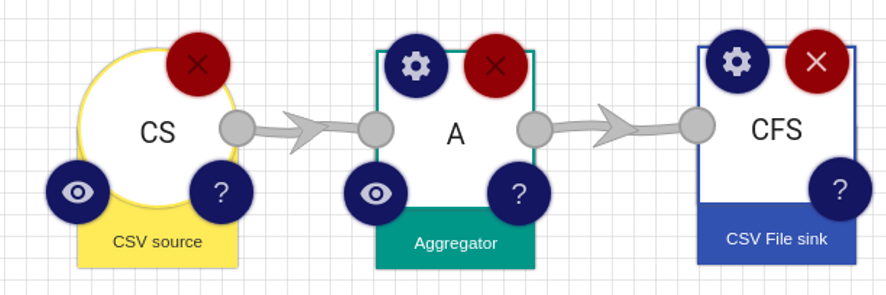
\includegraphics[width=\textwidth]{figures/visualizations/EvaluationPipelineSceenshot_1500.png}
    \caption{Screenshot of the test pipeline used throughout the evaluation}
    \label{fEvaluationPipeline}
\end{figure}

The test case used for the evaluation is the aforementioned \ref{cAggregation}. The needed \gls{pe}s were implemented in StreamPipes, and the pipeline was recreated, as shown in Figure \ref{fEvaluationPipeline}. Using \ref{cAggregation} as an illustrative case allows for a reliable way of determining whether the resulting output is consistent. The correct outcome is known since this pipeline is a composition of deterministic \gls{pe}s with a fixed input from a predefined \gls{csv} file. Any deviations from the expected output, which is also saved to a \gls{csv} file, flag inconsistent results.\par


\begin{figure}[!ht]
    \centering
    \graphicspath{{./figures/code/}}
    \includesvg[width=\textwidth]{figures/visualizations/EvaluationSetup_1500.svg}
    \caption{Setup for the evaluated experiments}
    \label{fEvaluationSetup}
\end{figure}


This test-case is evaluated on a setup of two devices, which are both connected to a local router via gigabit ethernet. The first device is a desktop PC with a 6-core, 3.60GHz AMD Ryzen 3600 processor with a total of 16GiB of RAM running Ubuntu 20.04. It simulates a centralized computing entity. A Raspberry Pi 4 single-board computer is deployed as the second device to simulate a small computing device in the fog. It is powered by a 4 core 1.50GHz ARM Cortex-A72 processor, has 4GiB of RAM, and runs a 64bit version of Raspberry Pi \gls{os} (a Debian based operating system optimized for the Raspberry Pi). For the evaluation of the test-case, the StreamPipes components are deployed, as depicted in Figure \ref{fEvaluationSetup}. The desktop PC hosts the micro-services mandatory for the StreamPipes deployment, namely Consul, Apache ActiveMQ, Apache Kafka, Apache ZooKeeper, InfluxDB, and Apache CouchDB, as well as the StreamPipes Backend and the user interface. These microservices are all deployed in independent but connected docker containers. Additionally to this base setup, the desktop PC hosts the source and sink \gls{pe}, as well as an instance of the aggregating \gls{pe}. The Raspberry Pi also hosts a containerized instance of the aggregating \gls{pe}.

\subsection{Results}
\label{lEvaluationResults}

Experiments \acrshort{e}1, \acrshort{e}2, and \acrshort{e}3 were conducted using the above-described test case on the test setup. The results of these experiments are presented in this sub-chapter.



\subsubsection{Pipeline Element Live Migration}
\label{lResultsOperatorStateMigration}

In the first experiment, the test case pipeline was set up using a source and sink \gls{pe} on the desktop PC and an aggregator \gls{pe} on the Raspberry Pi. Following a random wait time after starting the pipeline, the aggregator on the Raspberry Pi was migrated to the desktop PC using the \textit{\acrshort{pe} live migration}.\\
To simulate a real-world use case, this experiment was conducted while varying the network conditions and the state-size. The network conditions were varied to mimic the varying latencies encountered in fog computing \cite{Puliafito.2018}. This variation was realized by using the linux traffic control tools to add a network delay to traffic between the Raspberry Pi and the desktop PC. Three scenarios were distinguished. Tests with no added network delay (n0) (averaging a latency of 0.2ms between the devices), tests with an added network delay that is normally distributed averaging 100ms with a variance of 10ms (n100), and the last tests with a normally distributed network delay averaging 500ms with a variance of 50ms (n500), were conducted. State-sizes are the second varied factor. The variation of the state-size simulates different \gls{pe}s, whose states can have vastly different sizes. State-sizes range from sub-Kibibyte sizes, for example, in the aggregator used in the experiments, when it is configured to aggregate over a narrow window of past events, to state-sizes in the tens of \gls{mib}. For instance, a \gls{pe} that uses a machine learning model that changes over time due to reinforcement learning could have a larger state-size. The same aggregating \gls{pe} is used throughout all experiments and was therefore equipped with the capability to increase its state-size artificially. The state-size is increased by adding a String value with configurable length to the state. The experiment was conducted with three state-size setups. The first test-series was conducted with no added state (s0), the second one with 1\gls{mib} of added state (s1), and the last test-series with 5\gls{mib} of added state (s5).\par

In total, nine test-series were conducted, with differing network conditions and state-sizes between test-series. In all test-runs, the aggregating \gls{pe} was configured to aggregate the last ten values. The events were fed into the pipeline with an average frequency of one event every 300ms. Each test was performed ten times to achieve more reliable results.\par

\begin{figure}[!ht]
    \centering
    \subfloat[\centering Added average network delay of 0ms (n0)]{{\includesvg[width=5cm]{figures/statistics/OSMNetwork0_500.svg}}{\label{rOperatorStateMigrationNW0}}}%
    \subfloat[\centering Added average network delay of 100ms (n100)]{{\includesvg[width=5cm]{figures/statistics/OSMNetwork100_500.svg}}{\label{rOperatorStateMigrationNW100}}}%
    \subfloat[\centering Added average network delay of 500ms (n500)]{{\includesvg[width=5cm]{figures/statistics/OSMNetwork500_500.svg}}{\label{rOperatorStateMigrationNW500}}}%
    \captionsetup[subfloat]{labelformat=empty}
    \subfloat[\centering]{{\includesvg[width=15cm]{figures/statistics/OSMLegend_1500.svg}}}%
    
    \caption{Results of E1 under different networking conditions}%
    \label{rStateMigrationDuration}%
\end{figure}



Figure \ref{rStateMigrationDuration} depicts the total migration times for the different test-series. The total time is further broken down into 4 phases, corresponding to the migration procedure. In the first phase, the \gls{pe} is paused on the origin node. The current state is fetched from the \gls{pe} on the origin node in the second phase. In the third phase, the \gls{pe} is invoked on the target node with the previously fetched state. The migration is finalized by discarding the \gls{pe} on the origin node and saving the changed pipeline description. Since the \gls{pe} on the target node begins processing after its invocation, the sum of the first three phases provides an upper limit for the \gls{pe} downtime. The error bars in Figure \ref{rStateMigrationDuration} represent the standard deviation for the total time of migration.\\ 
In the test-series without added network delay (Figure \ref{rOperatorStateMigrationNW0}), the \gls{pe} downtime increased from 48ms with s0 to 112ms with s1 and further to 308ms with s5. In the test-series with an average of 100ms added network delay (Figure \ref{rOperatorStateMigrationNW100}), the \gls{pe} downtime rose from an average of 243ms with s0 to 911ms with s1 and 1278ms with s5. In the final test-series, with an average of 500ms added network delay (Figure \ref{rOperatorStateMigrationNW500}), the results increased similarly. They went from 1057ms with s0 to 2571ms at s1 and 3823ms at s5.\\
Overall, the results show two correlations. Firstly, the total time of migration and the \gls{pe} downtime both increase with an increasing state-size. Secondly, the total time of migration and the \gls{pe} downtime also increase with an increasing network delay. The phases whose duration increased the most with increasing state-size were phases 2 and 3. Across all network delays, the average duration of phase 2 rose by 540\% between tests with s0 and s1 and by 200\% between tests with s1 and s5. The average duration of phase 3 across all network delays increased by 150\% between tests with s0 and s1, and by 220\% between tests with s1 and s5. In contrast to these two phases, which involve handling the operator state, the duration of phases 1 and 4 did not change significantly in regards to the state-size. However, the duration of these two phases, together with phase 2 did rise with increasing network delay. The average duration of Phase 1 across all state-sizes rose by 1160\% between tests with n0 and n100, and by 490\% between tests with n100 and n500. A similar increase can be observed for phase 2, with an increase in duration by 880\% between tests with n0 and n100, and by 350\% between tests with n100 and n500. This relation can also be seen for phase 4, whose duration increases by 230\% between tests with n0 and n100, and by 360\% between tests with n100 and n500.\par

\begin{figure}[!ht]
    \centering
    \subfloat[\centering CPU load in an illustrative test case]{{\includesvg[width=7.5cm]{figures/statistics/OperatorStateMigrationCPUSingleCase_750.svg}}{\label{rOperatorStateMigrationCPUSingle}}}%
    \subfloat[\centering Average CPU load during \textit{\acrshort{pe} live migration}]{{\includesvg[width=7.5cm]{figures/statistics/OperatorStateMigrationCPUAverage_750.svg}}{\label{rOperatorStateMigrationCPUAverage}}}%
    \caption{CPU load in the \gls{pe}'s container on the Raspberry Pi}%
    \label{rOperatorStateMigrationCPU}%
\end{figure}


In addition to these measurements, the \gls{cpu} on the Raspberry Pi was monitored. Figure \ref{rOperatorStateMigrationCPUSingle} shows an illustrative test run with s5 and n0. The \gls{cpu} load is on a level of under 10\% for most of the time with three spikes of 40\% to 60\% at 2.4 seconds, 5.4 seconds, and 7.2 seconds. The first two spikes correspond with the timing of the checkpointing. The last spike coincides with the migration.\\
To further inspect the \gls{cpu} load during the migration, a follow-up test-series was conducted, for which the artificial state-size was increased to 50\gls{mib}. Figure \ref{rOperatorStateMigrationCPUAverage} shows the average \gls{cpu} load for the migration timeframe. During this timeframe, an increase in the \gls{cpu} load to 50\% was observed.\par

The last evaluated factor was the consistency of the results. The consistency was assessed by analyzing the output of the sink \gls{pe}. As previously explained, the expected output is deterministic. Therefore, the consistency check was conducted by comparing the sink output with the expected output. In a total of 110 evaluated runs, the result was always consistent. 
%This held true, even for an average time between events of xx and xx.

\subsubsection{Pipeline Element Restoration}
\label{lResultsOperatorStateRestoration}
For the second experiment, the test case pipeline was set up using a source, sink, and aggregator \gls{pe} on the desktop PE. After a random period of time, the aggregator on the desktop PC was discarded to simulate a \gls{pe} becoming interrupted. Thereafter, a random waiting period followed, after which the aggregator was restored on the Raspberry Pi using the \textit{\acrshort{pe} restoration}. Since checkpointing is done at regular intervals, the random timing of discarding the \gls{pe} leads to a variation in the number of events that need to be reprocessed. As the time period between discarding and restoring the \gls{pe} is also random, the number of intermediary events is also irregular. Intermediary events are the events occurring in the time between the interruption of the \gls{pe} and the start of the restoration (as described in section \ref{lMigrationConcept} Figure \ref{fTimingOSR}).\par

For this experiment, a total of 100 test runs were conducted. In all test-runs, the aggregating \gls{pe} was configured to aggregate the last ten values. The state-size was artificially increased by 1\gls{mib}. The events were fed into the pipeline with an average frequency of one event every 300ms. Additionally, the \gls{pe}-level checkpointing was configured to a frequency of checkpointing once every five seconds.\par


\begin{figure}[!ht]
    \centering
    \subfloat[\centering Duration of reprocessing in relation to the number of reprocessed events]{{\includesvg[width=7.5cm]{figures/statistics/StateRestorationScatterReprocess_750.svg}}{\label{rOperatorStateRestorationReprocessing}}}%
    \subfloat[\centering Duration of processing intermediate events in relation to the number of intermediately processed events]{{\includesvg[width=7.5cm]{figures/statistics/StateRestorationScatterIntermediate_750.svg}}{\label{rOperatorStateRestorationIntermediateProcessing}}}%
    \caption{Duration of reprocessing and intermediately processing events after \textit{\acrshort{pe} restoration}}%
    \label{rOperatorStateRestorationDuration}%
\end{figure}


Figure \ref{rOperatorStateRestorationDuration} displays the results of E2. In Figure \ref{rOperatorStateRestorationReprocessing}, the time spent reprocessing is depicted in dependence on the number of reprocessed events. The results show an increase in processing time with an increase in the number of reprocessed events. A similar relation can be observed between the time spent processing intermediary events and the number of intermediary processed events (Figure \ref{rOperatorStateRestorationIntermediateProcessing}). The average time per reprocessed event is 0.608ms, which is significantly lower than the average time per intermediary processed event, which takes 1.109ms on average. This difference can be attributed to the fact that the result of processing intermediary events is output by a Kafka producer, whereas the output of reprocessing is discarded.\par

\begin{figure}[!ht]
    \centering
    \graphicspath{{./figures/code/}}
    \includesvg[width=\textwidth]{figures/statistics/stateRestorationCPU_1500.svg}
    \caption{\gls{cpu} load in the \gls{pe}'s container on the Raspberry Pi for an illustrative test case}
    \label{rOperatorStateRestorationCPU}
\end{figure}

The \textit{\acrshort{pe} restoration} has a significant impact on the \gls{cpu} load. This is shown in Figure \ref{rOperatorStateRestorationCPU}, which depicts the \gls{cpu} load of the aggregating \gls{pe}'s container on the Raspberry Pi in a selected test-run. In the time between 0.338 seconds and 0.570 seconds, 191 events were reprocessed. After that, 309 intermediary events were processed until 1.120 seconds. Over this period, the \gls{cpu} load increased to around 90\%. Once regular event processing took over, the \gls{cpu} load dropped to under 10\%, where it leveled off.\par

To evaluate the consistency of the \textit{\acrshort{pe} restoration}, five additional test-runs were conducted. For these test runs, the setup was adjusted. Instead of initially deploying the test pipeline solely on the desktop PC, the aggregator was deployed on the Raspberry Pi. In the test-runs, the Raspberry Pi was forcefully interrupted by cutting off its power connection a random time period after the pipeline was started. Thereafter, a \textit{\acrshort{pe} restoration} with the desktop PC as target node was performed.\\
The resulting output of the five conducted test runs shows no inconsistencies.


\subsubsection{Checkpointing}
\label{lResultsCheckpointing}
The checkpointing performance was assessed based on the data gathered in E1. Figure \ref{rCheckpointingDuration} depicts the average time checkpointing the aggregator's operator state takes on the Raspberry Pi, depending on the additional state size. While the duration of checkpointing was only 3.1ms in the tests with no added state, the duration increased to 23.8ms at 1\gls{mib} of artificially added state and rose to 84.1ms with 5\gls{mib} of added state. The share of the serialization time in the total checkpointing duration also increased from 0.3\% with no added state to 32.3\% with 1\gls{mib} added state and further to 40.6\% with 5\gls{mib} added state. 

\begin{figure}[H]
    \centering
    \graphicspath{{./figures/code/}}
    \includesvg[width=11.1cm]{figures/statistics/CheckpointingTime_1110.svg}
    \caption{Checkpointing duration in relation to the operator state size}
    \label{rCheckpointingDuration}
\end{figure}


\subsection{Discussion}
\label{lDiscussion}

In this discussion, the implementation and the evaluation results are examined against the backdrop of the requirements. From thereon, the limitations of this thesis are derived.\par

\textbf{Basic Functionality}\par
The basic functionality required by the \ref{rBasicMigration} and the \ref{rRecovery} requirement is provided by the conceptual framework developed in \ref{lMigrationConcept}. The proof of concept implementation could satisfy these requirements throughout the experiments.\\
Therefore, the \ref{rBasicMigration} and the \ref{rRecovery} requirement are met.\par

\textbf{Problem Handling}\par
\ref{rProblemHandling} is another requirement concerning the migration functionality. While the \textit{\acrshort{pe} live migration} implementation addresses problem handling, the \textit{\acrshort{pe} restoration} does it only to a lesser extent. 
In the \textit{\acrshort{pe} live migration}, the \gls{pe} on the origin node is paused until the correct invocation on the target node is confirmed. Processing is restarted on the origin node if the \gls{pe} cannot be invoked on the target node, providing a safety measure for problems during the migration. The \textit{\acrshort{pe} restoration} implementation only informs about the restoration attempt's success or failure but does not provide any active measure to address problems.\\
Overall, the \ref{rProblemHandling} requirement is addressed partly by the conceptual framework. To fully meet this requirement, software components that orchestrate the migration (e.g., decide when and with which target to migrate) need to react to the feedback received from the migration procedures.\par


\textbf{Consistency}\par
Achieving an exactly-once semantic with a consistent output is the best-case scenario, according to the \ref{rConsistency} requirement. The \textit{\acrshort{pe} live migration} is implemented with the intention of an exactly-once semantic. The results of E1 showed no inconsistencies, providing evidence that the exactly-once semantic was achieved and that the operator state is migrated as desired.\\
The \textit{\acrshort{pe} restoration} implementation is designed to provide an at-least-once semantic, with the intention to avoid processing events a second time when possible. The preliminary results from E2 showed no inconsistencies, meaning that the correct operator state was reconstructed and that no event was not processed or processed twice (except for reprocessing, which does not output events).\\
Therefore, the consistency requirement was largely met. A possible further improvement of the \textit{\acrshort{pe} restoration} could be achieved with Apache Kafka as an intermediary message broker, using its in-build capabilities for exactly-once processing \cite{Narkhede.2017}. On the flip side, this would add additional overhead to event processing.\par

\textbf{\acrlong{pe} Downtime}\par
The \ref{rDowntime} requirement states that the \gls{pe} downtime should be as low as possible, which is addressed by the developed conceptual framework and the implementation. The evaluation results reveal factors that influence the \gls{pe} downtime in both the \textit{\acrshort{pe} live migration} and the \textit{\acrshort{pe} restoration}.\\
For the \textit{\acrshort{pe} live migration}, the results of E1 imply a positive correlation between state-size and migration duration (p=xx) and a positive correlation between network delay and migration duration. This increase in the migration duration also entails an increase in the \gls{pe} downtime.\\
In E2, the \textit{\acrshort{pe} restoration} was examined. A positive correlation between the number of reprocessed events and the reprocessing duration was observed (p<0.0001). A positive correlation was also found in the relation between the number of intermediate events processed and the duration of the intermediate processing of events (p<0.0001).\\
The information gathered in E1 reveals a potential for downtime improvement. A high \gls{pe} downtime can be attributed to network impairments and great state-sizes. In a situation where the origin node of the \gls{pe} that should be migrated suffers from a high network delay, it could be beneficial to restore the \gls{pe} on the target node from an old checkpoint using the \textit{\acrshort{pe} restoration} procedure (instead of \textit{\acrshort{pe} live migration}). The \textit{\acrshort{pe} restoration} is favorable if getting the checkpoint from the database and reprocessing events can be done faster than getting the \gls{pe}'s most recent state. However, the decision between the procedures additionally depends on the \gls{pe} in question since it can be suspected that different \gls{pe}s vary in their performance when reprocessing events. Thus, a holistic approach is needed to address this problem.\\
In conclusion, there is further potential to lower the \ref{rDowntime}, even though the \gls{pe} \ref{rDowntime} is considered in the proof of concept implementation. Using a holistic approach and applying the tactics proposed in related works could help to minimize the downtime.\par


\textbf{Development}\par
According to the \ref{rDevelopment} requirement, the migration capability should add as little effort as possible to the development of \gls{pe}s. This is addressed in the proof of concept implementation by providing the universal \textit{StateHandler}, which offers a convenient way for developers to expose the processing state. Additionally, the buffer and routing state are handled automatically.\\
Overall, the \ref{rDevelopment} requirement is predominantly met, only requiring a minor additional effort in the \gls{pe} development.\par


\textbf{Fog Compatibility}\par
The \ref{rFogCompatibility} requirement demands resource constraints and varying networking conditions in the fog to be addressed.\\
The influence of varying network conditions on the \textit{\acrshort{pe} live migration}, and all associated steps were examined in E1. The \textit{\acrshort{pe} live migration} was not susceptible to faults or inconsistencies with network delays between 0ms and 500ms. However, the network delay had a significant impact on the duration of the migration. By allowing workload mobility, the \gls{pe} migration gives the possibility to lower the latency by relocating \gls{pe}s to available nodes with lower latency.\\
The impact on \gls{cpu} load was investigated for \textit{\acrshort{pe} live migration} in E1 and for \textit{\acrshort{pe} restoration} in E2. The results in E1 showed an increased \gls{cpu} load of around 50\% during migration. In E2, the \gls{cpu} load was even higher during event reprocessing and intermediate processing, culminating at more than 90\%. These observations were made with a \gls{pe} deployed on a Raspberry Pi, simulating a fog node with limited computing capabilities. Even though the \gls{cpu} load increased during migration and checkpointing, these increases resembled short spikes that were limited to the duration of the respective action. During the tests, the Raspberry Pi's limited capabilities did not provoke faults in the migration procedure and did also not impact the result's consistency. Workload mobility enables \gls{pe} relocation based on resource constraints, which could allow a more balanced and effective resource usage across the devices deployed in the fog.\\
These preliminary results suggest that the developed proof of concept is deployable across devices with different computing capabilities and under varying networking conditions, meeting the \ref{rFogCompatibility} requirement.\par


All in all, the set requirements are predominantly met by the proof of concept implementation. Out of all requirements, the \ref{rProblemHandling} and the \ref{rDowntime} requirement show the most potential for further improvement.

\textbf{Limitations}\par

The limitations of this thesis can be categorized into the limitations of the developed conceptual framework, the limitations of the implementation, and the limitations of the evaluation.\par

A clear limitation of the developed conceptual framework is that it revolves around two distinct procedures, which address different cases. This is a limitation since it requires a preceding categorization of the current case to decide which procedure to choose.\\
Additionally, the conceptual framework is developed for a use case with a centralized orchestrator. The centralization in \gls{dlac} limits the possibility of decentralized fog computing because it creates a dependency on a centralized orchestrator and a centralized database to provide globally available checkpoints.\par

The implementation is limited by technology dependency, missing handling of interrupted \gls{pe}s, and compatibility constraints.\\
A dependency exists to Apache Kafka because the implementation relies on its integrated offset management to handle the buffer state. This technology dependency could be addressed by persisting the buffer state, or even the whole operator state to the upstream \gls{pe}, as proposed by Fernandez et al. \cite{CastroFernandez.2013}.\\
Additionally, the implementation lacks measures to handle interrupted \gls{pe}s. However, these measures are needed to guarantee that a supposedly interrupted \gls{pe} does not come back to life, meaning that it does not start processing events again. A \gls{pe} coming back to life is undesirable because it would most certainly introduce inconsistencies in the resulting output event stream. Therefore, it needs to be discarded in such a case. One scenario where this could happen is when a \gls{pe} is restored on a new node because of temporary networking problems on its origin node. If the \gls{pe} on the origin node reconnects to the network, it might start processing events again.\\
Furthermore, the proof of concept implementation cannot be deployed on devices with a 32-bit arm processor. This is due to RocksDB, which only supports arm processors with a 64-bit architecture that supports the "AArch64" instruction set. This can be problematic since small computing devices used as fog nodes might have an insufficient arm processor.\par

Due to the high number of possibly influencing variables on the implementation's performance, only a selection of them could be examined in the evaluation.\\
Neither E1, nor E2 addresses other components of varying networking conditions than latency. For example, packet loss could also be problematic in the context of fog computing.\\
Another apparent weakness of the evaluation is that only experiments in a single test scenario and with a single \gls{pe} were conducted. This neglects the differences between \gls{pe}s, ranging from the complexity of the processing state to the effort needed to process events. These factors can be expected to influence the invocation time from an old state, as well as the reprocessing duration.\\
Lastly, the evaluation was conducted in a highly controlled environment. To determine the real-world performance, more realistic test scenarios need to be explored, for example, \ref{cMedical}.\par

\section{Conclusion}
\label{lConclusion}

\subsection{Summary}
\label{lSummary}

This work addressed the consistent migration of stream processing \gls{pe}s between nodes in the fog. This was motivated by outlining the need for \gls{pe} migration in fog computing applications to address a multitude of characteristic constraints and requirements in fog computing. The migration allows for workload mobility, which can be utilized to minimize latency, react to resource constraints, or address privacy issues. This becomes increasingly important with the proliferation of connected \gls{iot} devices, which can significantly profit from fog computing.\par

To lay the groundwork, the background section focused on the intricacies of fog computing and event-based stream processing. After introducing the concept of stateful and stateless \gls{pe}s, the operator state was introduced as a proper representation of state for the use case of stream-processing. The operator state is composed of the routing, processing, and buffer state. This abstraction serves to describe the state of stream processing \gls{pe}s.\par

Other works addressing the migration of stateful applications in the fog were subsequently presented. While early research focused on live migration of \gls{vm}s, more recently, the focus shifted to the migration of containerized applications, which proves to be less resource-intensive and better suited for the migration of applications in the fog. Some authors take a different approach by utilizing explicit state-management at the application-level, instead of migrating the whole operating system with the applications. These approaches resemble the ones introduced in the literature concerning state-management in data processing, which was thoroughly examined next. In these works, state is used not only for migration but also to provide scalability and fault tolerance.\par

Based on the related works, a conceptual framework addressing the research questions was developed. It adopts application-level state-management and addresses the requirements emerging from the research questions. The migration of running and interrupted \gls{pe}s are treated separately. The migration of a running \gls{pe} uses the current operator state, which is obtained from the \gls{pe} on the origin node, to start the \gls{pe} on the target node. This means that processing can be picked up on the target node at the same point it was interrupted on the origin node. In contrast, the migration of an interrupted \gls{pe} (a \gls{pe} that is unreachable) is performed using a previously acquired checkpoint of the \gls{pe}'s state. This checkpoint is used to restart the \gls{pe} on the target node and to recreate the correct operator state. Checkpoints are obtained through \gls{dlac}, which addresses \gls{pe} availability, fault tolerance, and global checkpoint availability by combining periodic asynchronous local checkpointing with periodic asynchronous global checkpointing.\par

As proof of concept, the developed conceptual framework was implemented into Apache StreamPipes in chapter \ref{lImplementation}. At first, the fundamental modifications and extensions to StreamPipes, enabling the migration, were implemented. Next, the implementation of the \textit{\acrshort{pe} live migration}, and the \textit{\acrshort{pe} restoration} procedure was presented. The implementation addresses the requirements set in the previous chapter and shows a possible realization of the conceptual framework, addressing different challenges that are not covered by the conceptual framework.\par

This implemented proof of concept was evaluated in three experiments. The first experiment evaluated the \textit{\acrshort{pe} live migration} and showed that increased network delay and bigger state sizes impact the \gls{pe} downtime and the overall migration duration. However, a negative effect on the consistency of the results could not be observed. In the next experiment, the \textit{\acrshort{pe} restoration} was examined. The results revealed a correlation between the number of events to be reprocessed and the duration of reprocessing. A similar correlation was observed between the number of intermediary events to be processed and the duration of processing them. The third experiment examined the checkpointing performance for different state sizes. The results show that the share of the processing state serialization in the checkpointing duration increased with the state-size.\\
After that, the acquired results were discussed, and the limitations of this thesis were outlined. In the discussion, it was established that the implementation does predominantly satisfy the requirements. Shortcomings were laid out in the limitations section.\\
In this chapter, this thesis is contrasted against related works. After that, the limitations are followed up with suggestions for future research that could expand on this thesis.\par


This thesis expands on related work by proposing a conceptual framework for the migration of stream-processing \gls{pe}s in the fog.\\
The application-level approach proposed in this thesis represents a contrast to the virtualization level migration approaches taken in the majority of works on the migration of applications in the fog. The choice of virtualization level approaches can be attributed to their generality. As elaborated on in chapter \ref{lMigrationConcept}, the virtualization level approaches facilitate this generality. However, using an application-level approach in the use case of stream processing allows addressing intricacies of stream processing \gls{pe}s. This facilitates the fulfillment of the requirements.\\
While the works concerning state in data processing deploy application-level approaches for state handling, they do not address fog computing specific requirements. Additionally, only a small fraction of these works address the migration of the operator state, while most others focus on providing fault tolerance and scalability. This thesis combines measures for fault tolerance with a concept for the migration while addressing fog specific requirements at the same time.



\subsection{Future Work}
\label{lFutureWork}

During the writing of this thesis, several topics for future work were identified. Most of these topics have already been broached in the Discussion section (\ref{lDiscussion}).\\
Future research could explore the transfer of the developed conceptual framework to a more decentralized setting, without a centralized node that handles the global availability of state backups. This could be realized by distributing the state checkpoints to other nodes hosting \gls{pe}s, as proposed by Fernandez et al. \cite{CastroFernandez.2013}.\\
A logical next step to improve the conceptual framework and the implementation is to unify the \textit{\acrshort{pe} live migration} and the \textit{\acrshort{pe} restoration}. This would also allow for a performance improvement, as elaborated on in chapter \ref{lDiscussion}.\\
Before the implementation of the \textit{\acrshort{pe} restoration} is used, the handling of interrupted \gls{pe}s should be addressed. It is essential to guarantee that a supposedly interrupted \gls{pe} does not come back to life, meaning that it does not start processing events again.\\
The implementation could be tested and examined in a test scenario closer to a real-world application and under variation of factors not yet investigated in the evaluation to achieve a more comprehensive evaluation.\\
Moreover, future work in general should assess the migration of applications in fog computing further, developing a more general approach that allows the migration of stream processing \gls{pe}s and further applications.
% ...usw.



% Anhang / Appendix
\appendix % Ab hier wird mit A, B, ... weiternummeriert.
% Für den Fall eines Anhangs entkommentieren
\section{Appendix}
\subsection{Search interest in IoT}
\label{lSearchInterestInIoT}
\begin{table}[!h]
    \begin{tabular}{|p{2.6cm}||p{0.9cm}|p{0.9cm}|p{0.9cm}|p{0.9cm}|p{0.9cm}|p{0.9cm}|p{0.9cm}|p{0.9cm}|p{0.9cm}|p{0.9cm}|p{0.9cm}|}
    \hline
     Year&2009&2010&2011&2012&2013&2014&2015&2016&2017&2018&2019\\ 
     \hline
     Average search interest&9,17&13,92&11,58&9,92&11,45&25,42&52,42&78,08&90,00&91,25&90,42\\
     \hline
    \end{tabular}
    \caption{Worldwide search interest for the topic of "Internet of Things" according to data from Google Trends. Yearly average for the years 2009-2019.}
    \label{tSearchInterestIoT}
\end{table}


% Literaturverzeichnis
\bibliographystyle{acm}
\bibliography{references} % Datei mit Literaturangaben einbinden

% Schriftliche Erklärung
\newpage
\mbox{}\thispagestyle{empty}

\vspace*{1cm}

{\Large \textbf{\ifthenelse{\boolean{english}}{Assertion}{Erklärung}}} 

\bigskip

\ifthenelse{\boolean{english}}
{\selectlanguage{english}
\textit{Ich versichere wahrheitsgemäß, die Arbeit selbstständig verfasst, alle benutzten Hilfsmittel vollständig und genau angegeben und alles kenntlich gemacht zu haben, was aus Arbeiten anderer unverändert oder mit Abänderungen entnommen wurde sowie die Satzung des KIT zur Sicherung guter wissenschaftlicher Praxis in der jeweils gültigen Fassung beachtet zu haben.}}
{\selectlanguage{ngerman}
\textit{Ich versichere wahrheitsgemäß, die Arbeit selbstständig verfasst, alle benutzten Hilfsmittel vollständig und genau angegeben und alles kenntlich gemacht zu haben, was aus Arbeiten anderer unverändert oder mit Abänderungen entnommen wurde sowie die Satzung des KIT zur Sicherung guter wissenschaftlicher Praxis in der jeweils gültigen Fassung beachtet zu haben.}}

\vspace{1cm}

%
%WICHTIG: Prüfen Sie unbedingt, ob der Text der Erklärung mit der jeweils für den Studiengang aktuell gültigen SPO übereinstimmt!
%
%TODO: Datum der Erklärung angeben
%            Hinweis: Das Datum der Erklärung ist üblicherweise das Abgabedatum
%
%TODO: Eigenen Vornamen und Nachnamen angeben
%
Karlsruhe, \today \hfill Daniel Gomm

%\thispagestyle{empty}\cleardoublepage

%\mbox{}\thispagestyle{empty}


\end{document}